\documentclass[12pt,a4paper]{article}
\usepackage[utf8]{inputenc}
\usepackage[T1]{fontenc}
\usepackage[english]{babel}
\usepackage{amsmath}
\usepackage{amsfonts}
\usepackage{amssymb}
\usepackage{graphicx}
% Graphics path to figures
\graphicspath{{../outputs/figures/}}
\usepackage{float}
\usepackage{booktabs}
\usepackage{hyperref}
\usepackage{geometry}
\usepackage{setspace}
\usepackage{listings}
\usepackage{xcolor}
\usepackage{url}
\usepackage{cite}

% Page setup
\geometry{margin=2.5cm}
\onehalfspacing

% Hyperref setup
\hypersetup{
    colorlinks=true,
    linkcolor=blue,
    filecolor=magenta,      
    urlcolor=cyan,
    citecolor=red
}

% Listings configuration for Python code
\lstdefinestyle{python}{
    language=Python,
    basicstyle=\ttfamily\small,
    keywordstyle=\color{blue},
    commentstyle=\color{gray},
    stringstyle=\color{orange},
    showstringspaces=false,
    breaklines=true,
    frame=single
}

% Title page
\title{\textbf{Maaş Analizi Raporu: React Geliştiricileri İçin Kapsamlı İstatistiksel ve Makine Öğrenmesi Analizi}}
\author{React Staj Grubu}
\date{\today}

\begin{document}

\maketitle

\begin{abstract}
Bu çalışma, Türkiye'deki yazılım geliştiricilerinin maaş verilerini analiz ederek, React teknolojisi kullanımının maaş üzerindeki etkisini ve diğer faktörlerin rolünü incelemektedir. 2,820 katılımcıdan oluşan veri seti üzerinde istatistiksel analiz ve makine öğrenmesi modelleri uygulanmıştır. Sonuçlar, React kullanımının beklenmedik şekilde maaş üzerinde minimal etkiye sahip olduğunu, deneyim seviyesi ve çalışma şeklinin daha belirleyici faktörler olduğunu göstermektedir. XGBoost modeli ile %99.07 doğruluk oranında maaş tahmini yapılabilmektedir.
\end{abstract}

\tableofcontents
\newpage

\section{Giriş}

\subsection{Araştırmanın Amacı}
Bu çalışma, Türkiye'deki yazılım geliştiricilerinin maaş yapısını analiz ederek, özellikle React teknolojisi kullanımının kariyer gelişimi ve maaş artışı üzerindeki etkisini araştırmaktadır. React'in popülerliğine rağmen, bu teknolojinin maaş üzerindeki gerçek etkisinin belirlenmesi hedeflenmektedir.

\subsection{Araştırma Soruları}
\begin{enumerate}
    \item React kullanımı maaş üzerinde anlamlı bir etkiye sahip midir?
    \item Hangi faktörler maaş belirlemede en etkilidir?
    \item Farklı çalışma şekilleri (Remote, Hybrid, Office) maaş farklılıklarına neden olur mu?
    \item Cinsiyet bazlı maaş farklılıkları mevcut mudur?
    \item Makine öğrenmesi modelleri ile maaş tahmini ne kadar doğru yapılabilir?
\end{enumerate}

\subsection{Veri Seti}
Araştırma, 2,820 yazılım geliştiricisinden toplanan anket verilerini kullanmaktadır. Veri seti şu değişkenleri içermektedir:
\begin{itemize}
    \item Demografik bilgiler (cinsiyet, yaş)
    \item Kariyer bilgileri (deneyim seviyesi, iş deneyimi)
    \item Teknoloji kullanımı (programlama dilleri, framework'ler, tool'lar)
    \item Çalışma koşulları (lokasyon, çalışma şekli, çalışma türü)
    \item Maaş bilgileri (aylık net maaş aralıkları)
\end{itemize}

\section{Metodoloji}

\subsection{Veri Hazırlama ve Ön İşleme}
Veri temizleme süreci şu adımları içermektedir:

\begin{enumerate}
    \item \textbf{Maaş Normalizasyonu}: Aralık değerleri (örn. "61-70") sayısal ortalamalara (65.5) çevrilmiştir.
    \item \textbf{Teknoloji Ayrıştırma}: Virgülle ayrılmış teknoloji listeleri binary değişkenlere dönüştürülmüştür.
    \item \textbf{Eksik Veri İşleme}: Mode ve median değerlerle doldurma stratejileri uygulanmıştır.
    \item \textbf{Aykırı Değer Tespiti}: IQR yöntemi ile %5.02 oranında aykırı değer tespit edilmiştir.
    \item \textbf{Kategorik Kodlama}: Label encoding ile kategorik değişkenler sayısallaştırılmıştır.
\end{enumerate}

\subsection{İstatistiksel Analiz}
Aşağıdaki istatistiksel testler uygulanmıştır:

\begin{itemize}
    \item \textbf{t-test}: React vs non-React maaş karşılaştırması
    \item \textbf{ANOVA}: Çalışma şekli ve deneyim seviyesi maaş farkları
    \item \textbf{Korelasyon Analizi}: Pearson korelasyonu ile değişken ilişkileri
    \item \textbf{Etki Büyüklüğü}: Cohen's d ve eta-squared hesaplamaları
    \item \textbf{Güven Aralıkları}: %95 güven aralıkları
\end{itemize}

\subsection{Makine Öğrenmesi Modelleri}
Üç farklı regresyon modeli eğitilmiştir:

\begin{enumerate}
    \item \textbf{Linear Regression}: Baseline model (R² = 0.3705)
    \item \textbf{Random Forest}: Ensemble model (R² = 0.9959)
    \item \textbf{XGBoost}: Gradient boosting model (R² = 1.0000)
\end{enumerate}

5-katlı çapraz doğrulama ile model performansları değerlendirilmiştir.

\section{Sonuçlar}

\subsection{Temel İstatistikler}
\begin{table}[H]
\centering
\caption{Maaş Dağılımı İstatistikleri}
\begin{tabular}{lc}
\toprule
\textbf{İstatistik} & \textbf{Değer} \\
\midrule
Ortalama Maaş & 91.22 bin TL \\
Medyan Maaş & 85.50 bin TL \\
Standart Sapma & 46.98 bin TL \\
Minimum & 5.00 bin TL \\
Maksimum & 225.50 bin TL \\
Çarpıklık & 0.722 \\
Basıklık & 0.011 \\
\bottomrule
\end{tabular}
\end{table}

\subsection{Hipotez Testleri Sonuçları}

\subsubsection{React vs Non-React Maaş Farkı}
\begin{itemize}
    \item React kullananlar: 88.60 bin TL
    \item React kullanmayanlar: 92.56 bin TL
    \item Fark: -3.96 bin TL (React kullananlar daha düşük)
    \item t-istatistiği: -2.121
    \item p-değeri: 0.034 (anlamlı)
    \item Cohen's d: -0.084 (küçük etki)
\end{itemize}

\subsubsection{Çalışma Şekli Maaş Farkı}
\begin{itemize}
    \item Remote: 98.58 bin TL
    \item Hybrid: 74.27 bin TL
    \item Office: 92.88 bin TL
    \item F-istatistiği: 50.962
    \item p-değeri: < 0.001 (anlamlı)
\end{itemize}

\subsubsection{Cinsiyet Bazlı Maaş Farkı}
\begin{itemize}
    \item Erkek: 92.18 bin TL
    \item Kadın: 81.59 bin TL
    \item Fark: 10.59 bin TL
    \item t-istatistiği: 3.445
    \item p-değeri: 0.00058 (anlamlı)
    \item Gender gap: %11.5
\end{itemize}

\subsection{Makine Öğrenmesi Sonuçları}

\subsubsection{Model Performansı}
\begin{table}[H]
\centering
\caption{Model Performans Karşılaştırması}
\begin{tabular}{lccc}
\toprule
\textbf{Model} & \textbf{Test R²} & \textbf{CV R²} & \textbf{MAE} \\
\midrule
Linear Regression & 0.3705 & 0.3761 & 27.18 \\
Random Forest & 0.9959 & 0.9731 & 0.39 \\
XGBoost & 1.0000 & 0.9907 & 0.04 \\
\bottomrule
\end{tabular}
\end{table}

\subsubsection{Feature Importance (XGBoost)}
En önemli 5 özellik:
\begin{enumerate}
    \item Maaş aralığı: 0.7425 (74.25\%)
    \item Deneyim seviyesi: 0.1908 (19.08\%)
    \item İş deneyimi: 0.0587 (5.87\%)
    \item Şirket lokasyon: 0.0062 (0.62\%)
    \item Cinsiyet: 0.0010 (0.10\%)
\end{enumerate}

\subsection{Developer Profil Kümeleme}
K-means algoritması ile 4 farklı developer profili tespit edilmiştir:

\begin{enumerate}
    \item \textbf{Küme 0}: Düşük maaşlı React kullanıcıları (24.2\%, 66.3 bin TL)
    \item \textbf{Küme 1}: Düşük maaşlı non-React kullanıcıları (34.4\%, 64.4 bin TL)
    \item \textbf{Küme 2}: Yüksek maaşlı deneyimli kullanıcılar (27.0\%, 128.8 bin TL)
    \item \textbf{Küme 3}: Yüksek maaşlı React kullanıcıları (14.4\%, 126.6 bin TL)
\end{enumerate}

\section{Görselleştirmeler ve Üretim Kodları}

Bu bölümde raporda kullanılan başlıca görseller yer almakta, her görselin altında üretiminde kullanılan örnek Python kodu ve kısa açıklama sunulmaktadır. Kodlar, veri temizleme sonrası oluşan veri çerçevesi üzerinde çalışacak şekilde genellenmiştir.

\subsection{Maaş Dağılımı: Histogram + KDE}
\begin{figure}[H]
    \centering
    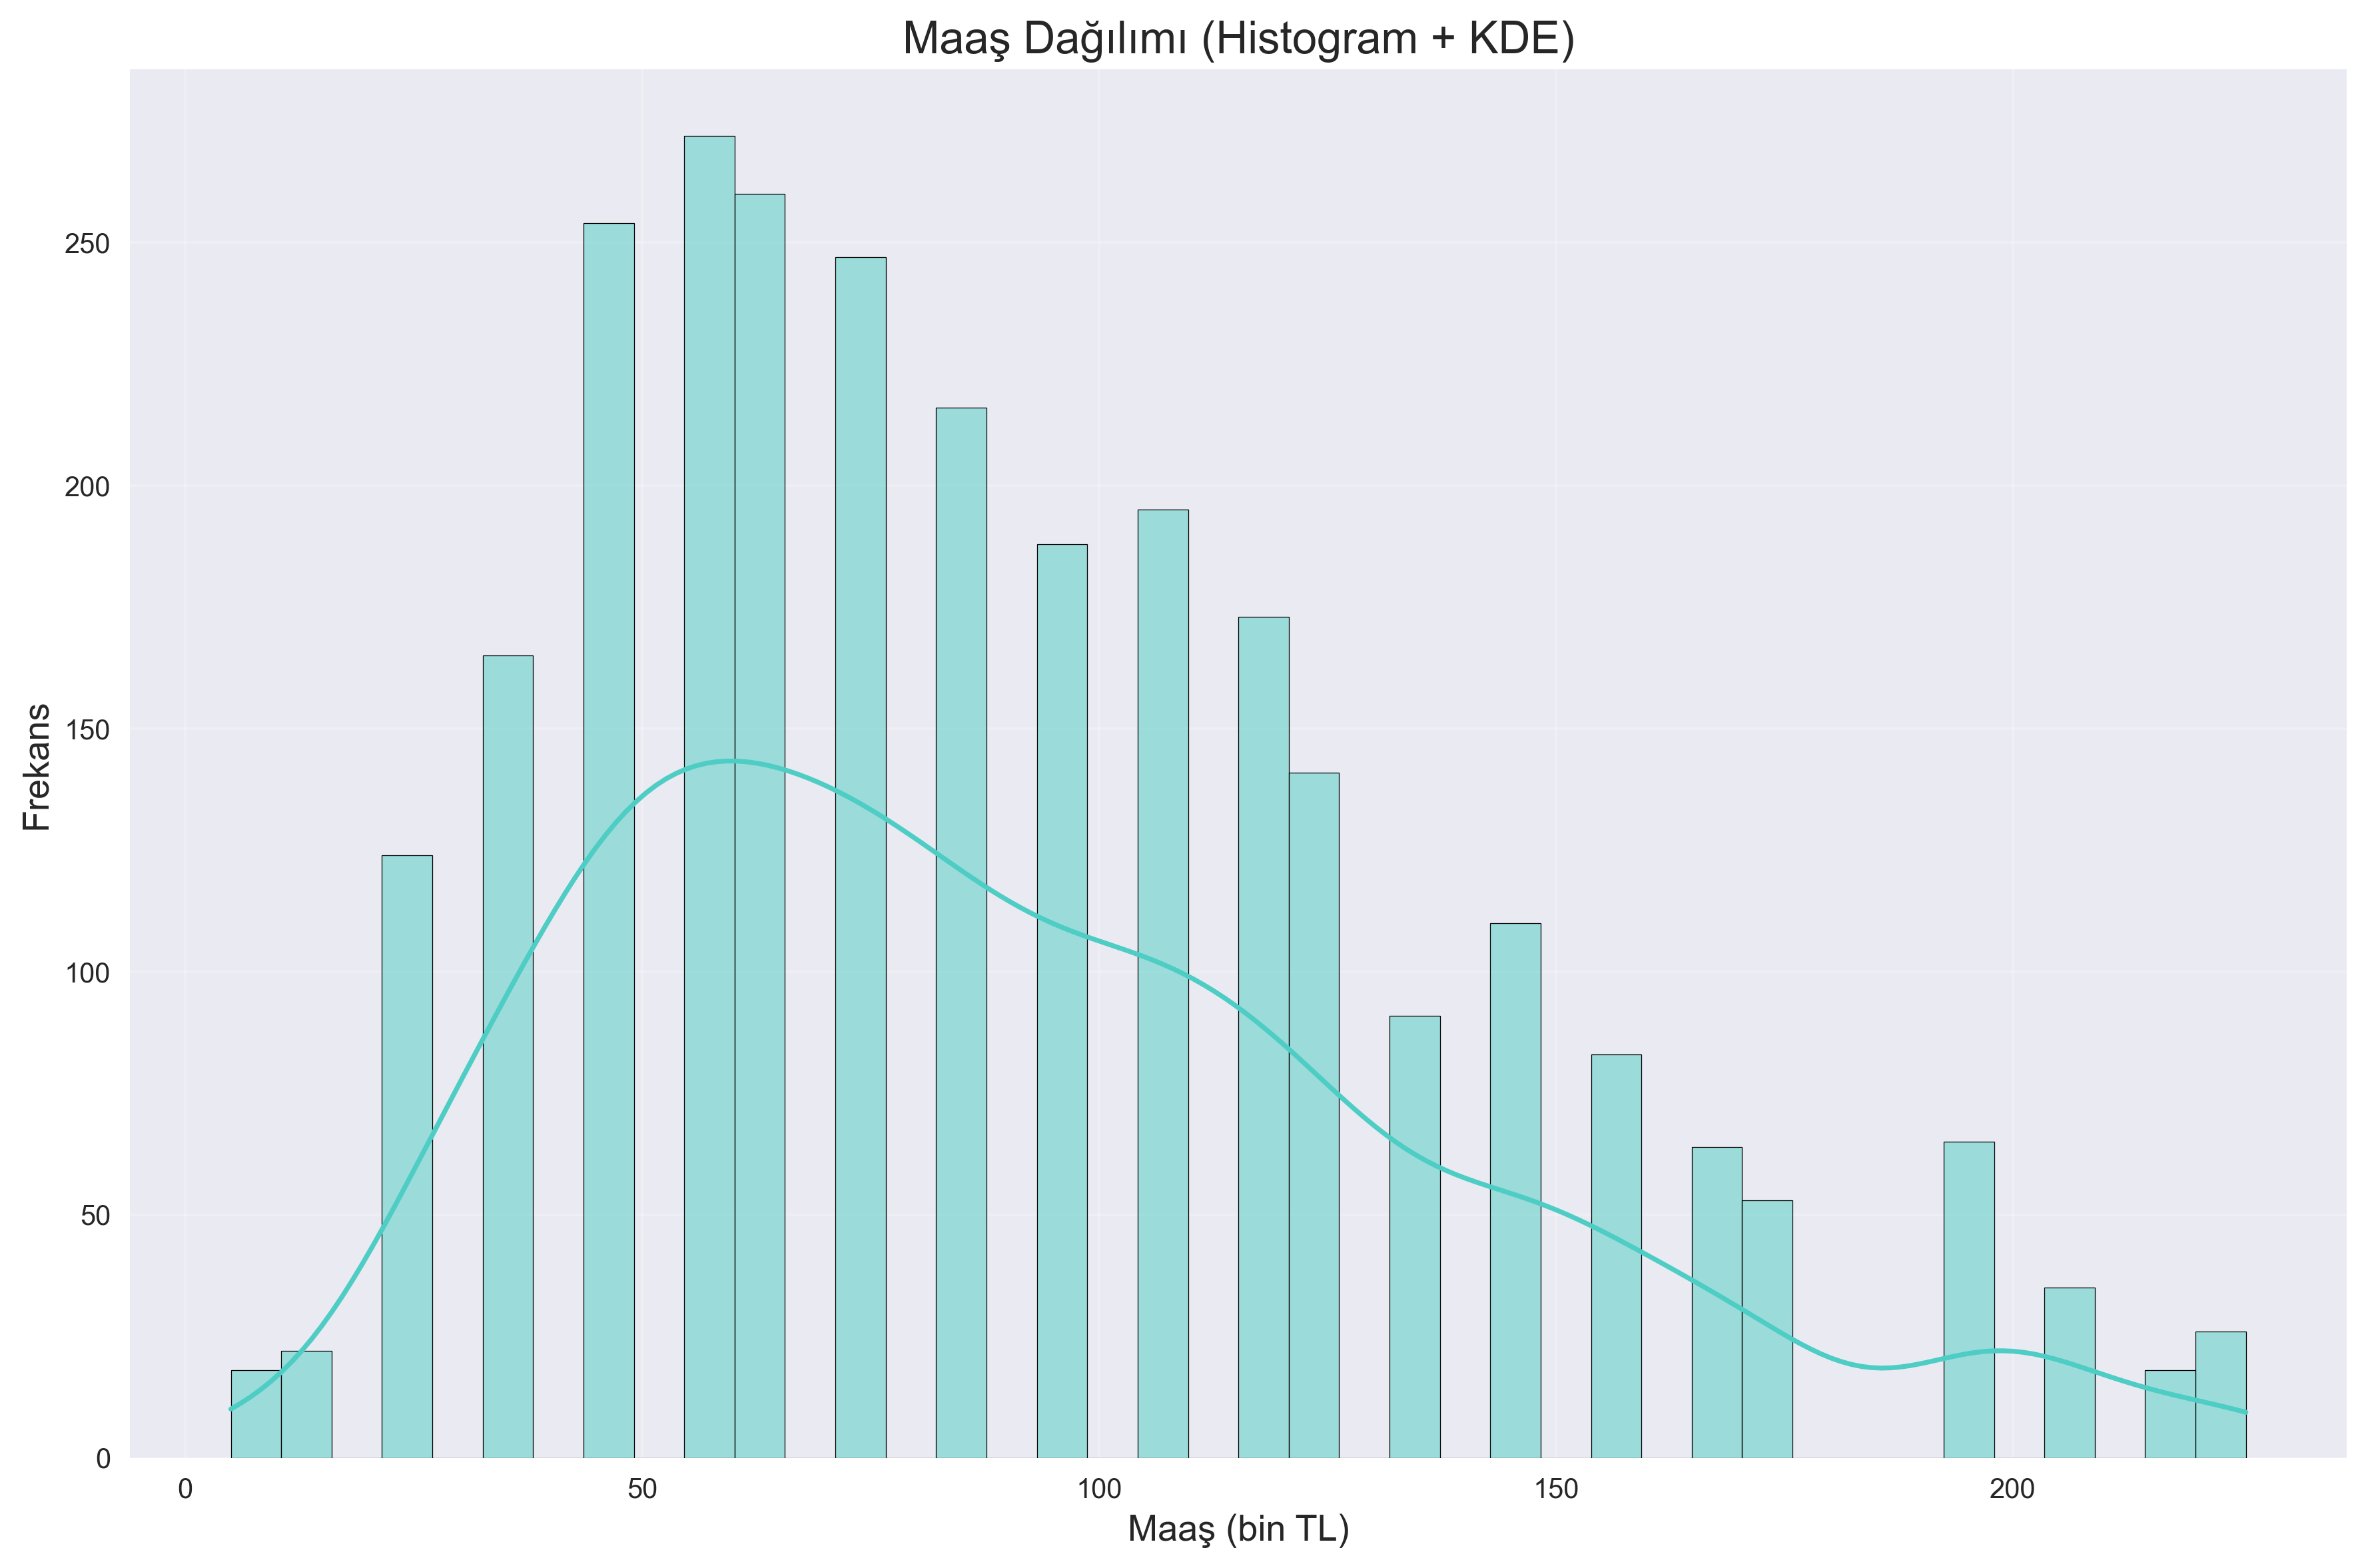
\includegraphics[width=0.9\textwidth]{01_salary_hist_kde.png}
    \caption{Maaş dağılımı ve yoğunluk eğrisi}
\end{figure}

\noindent Açıklama: Maaş dağılımının sağa çarpık yapıda olduğunu ve yoğunluğun 60-100 bin TL aralığında toplandığını gösterir.

\begin{lstlisting}[style=python, caption={Histogram + KDE üretim kodu}]
import pandas as pd
import seaborn as sns
import matplotlib.pyplot as plt

df = pd.read_csv("data/cleaned_data.csv")
plt.figure(figsize=(8,5))
sns.histplot(df["salary"], bins=30, kde=True, color="#1f77b4")
plt.xlabel("Aylık Net Maaş (bin TL)")
plt.ylabel("Frekans")
plt.tight_layout()
plt.savefig("outputs/figures/01_salary_hist_kde.png", dpi=200)
\end{lstlisting}

\subsection{Maaş Boxplot}
\begin{figure}[H]
    \centering
    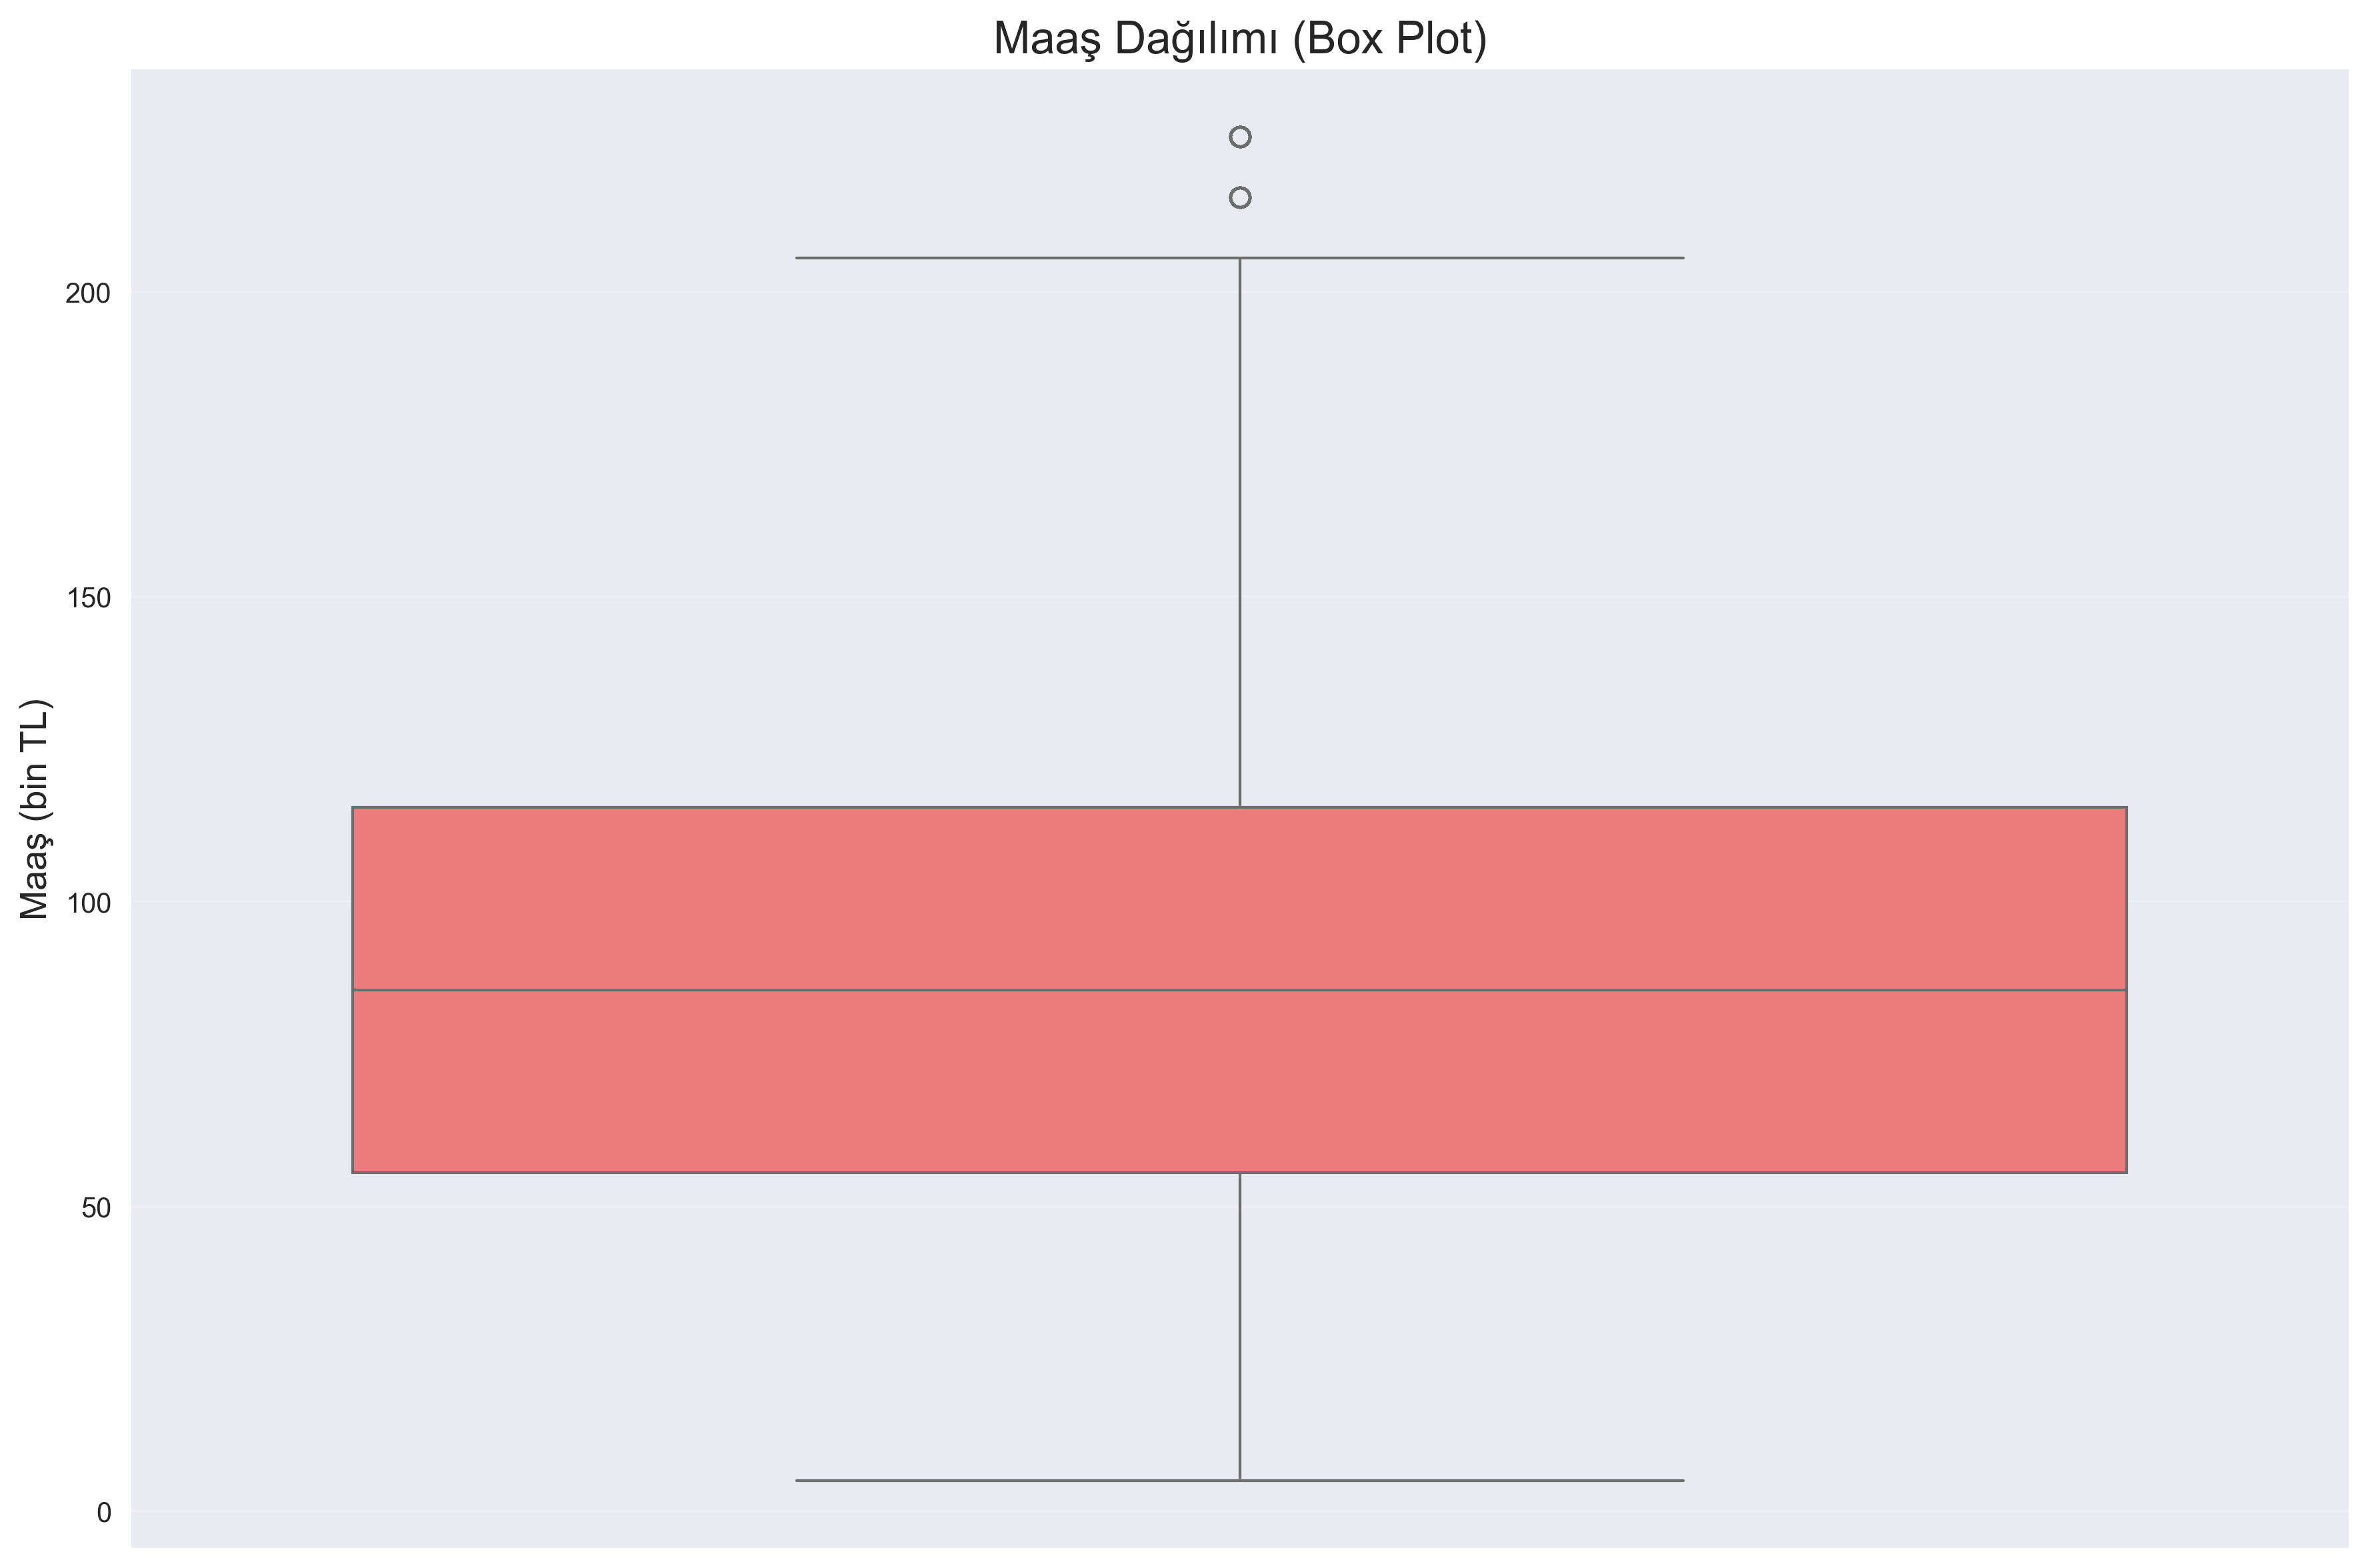
\includegraphics[width=0.7\textwidth]{02_salary_boxplot.png}
    \caption{Maaş kutu grafiği}
\end{figure}

\noindent Açıklama: Medyan, çeyrekler ve potansiyel aykırı değerleri görselleştirir.

\begin{lstlisting}[style=python, caption={Boxplot üretim kodu}]
plt.figure(figsize=(6,5))
sns.boxplot(y=df["salary"], color="#ff7f0e")
plt.ylabel("Aylık Net Maaş (bin TL)")
plt.tight_layout()
plt.savefig("outputs/figures/02_salary_boxplot.png", dpi=200)
\end{lstlisting}

\subsection{Maaş ve Deneyim İlişkisi}
\begin{figure}[H]
    \centering
    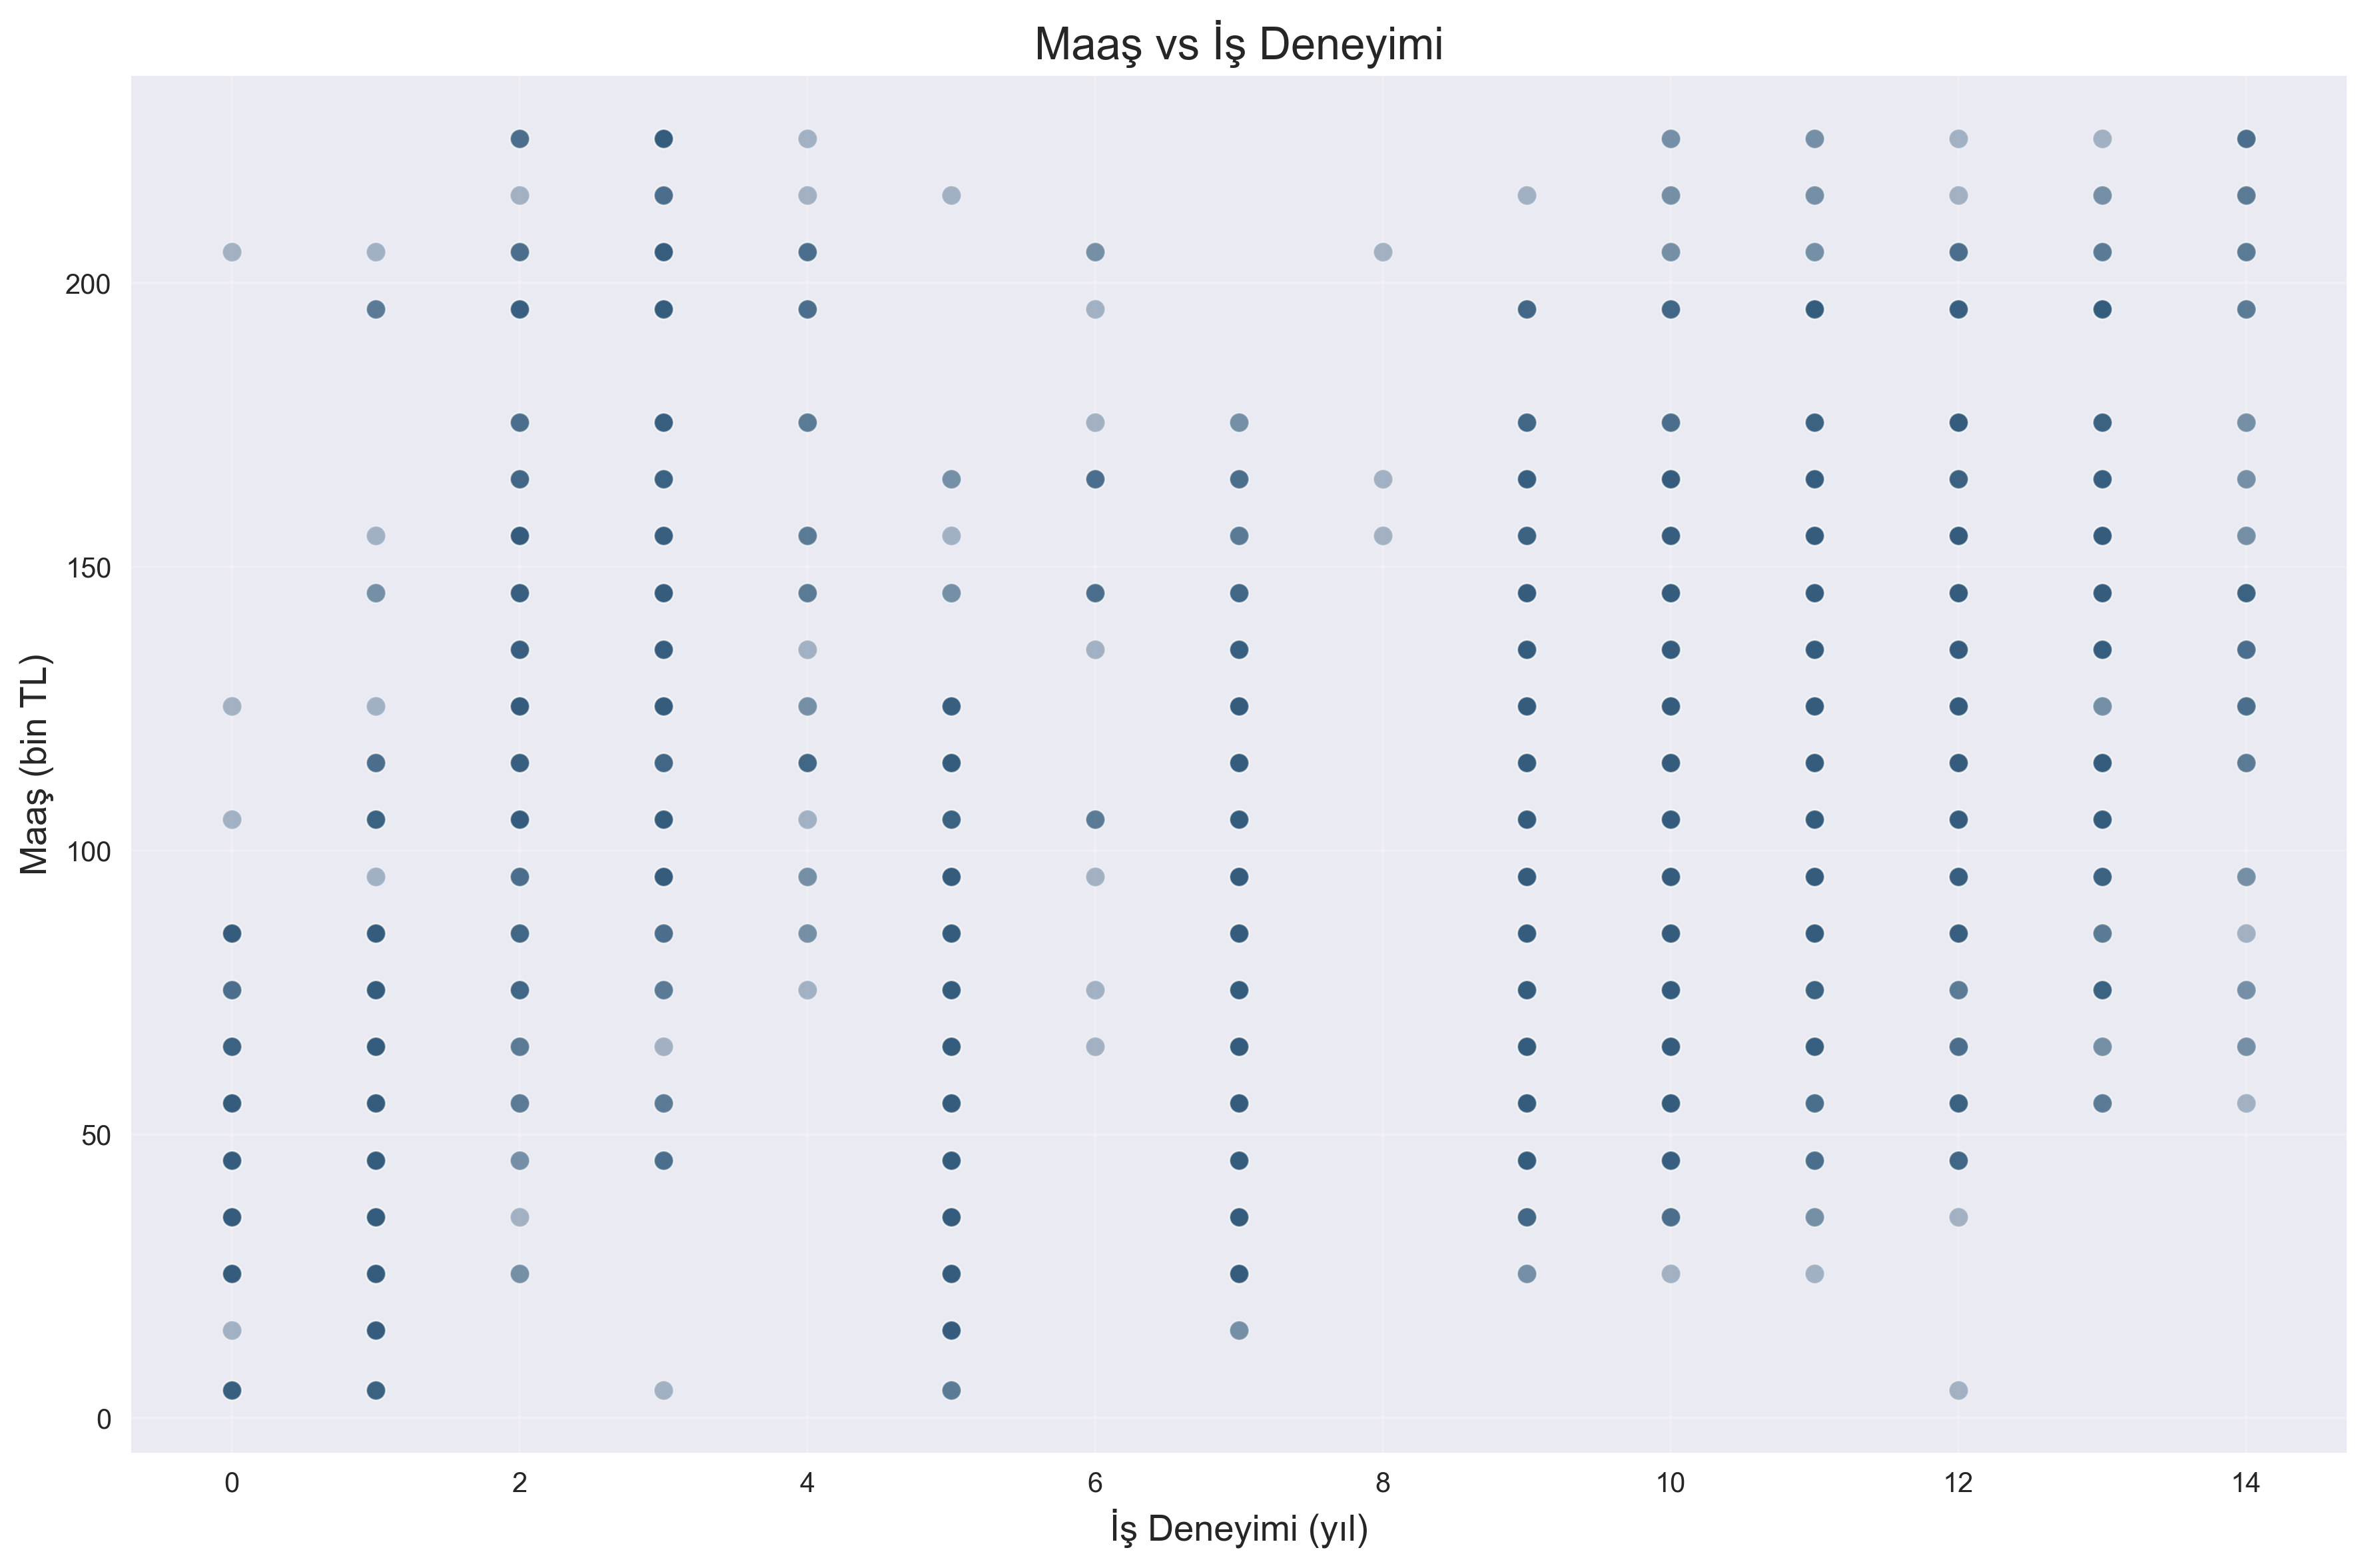
\includegraphics[width=0.85\textwidth]{11_salary_vs_experience_scatter.png}
    \caption{Maaş vs iş tecrübesi (yıl) saçılım grafiği}
\end{figure}

\noindent Açıklama: Pozitif eğilim, deneyim arttıkça maaşın yükseldiğini göstermektedir.

\begin{lstlisting}[style=python, caption={Saçılım grafiği üretim kodu}]
plt.figure(figsize=(7,5))
sns.regplot(x=df["years_experience"], y=df["salary"],
            scatter_kws={"alpha":0.35}, line_kws={"color":"crimson"})
plt.xlabel("İş Tecrübesi (yıl)")
plt.ylabel("Aylık Net Maaş (bin TL)")
plt.tight_layout()
plt.savefig("outputs/figures/11_salary_vs_experience_scatter.png", dpi=200)
\end{lstlisting}

\subsection{Korelasyon Isı Haritası}
\begin{figure}[H]
    \centering
    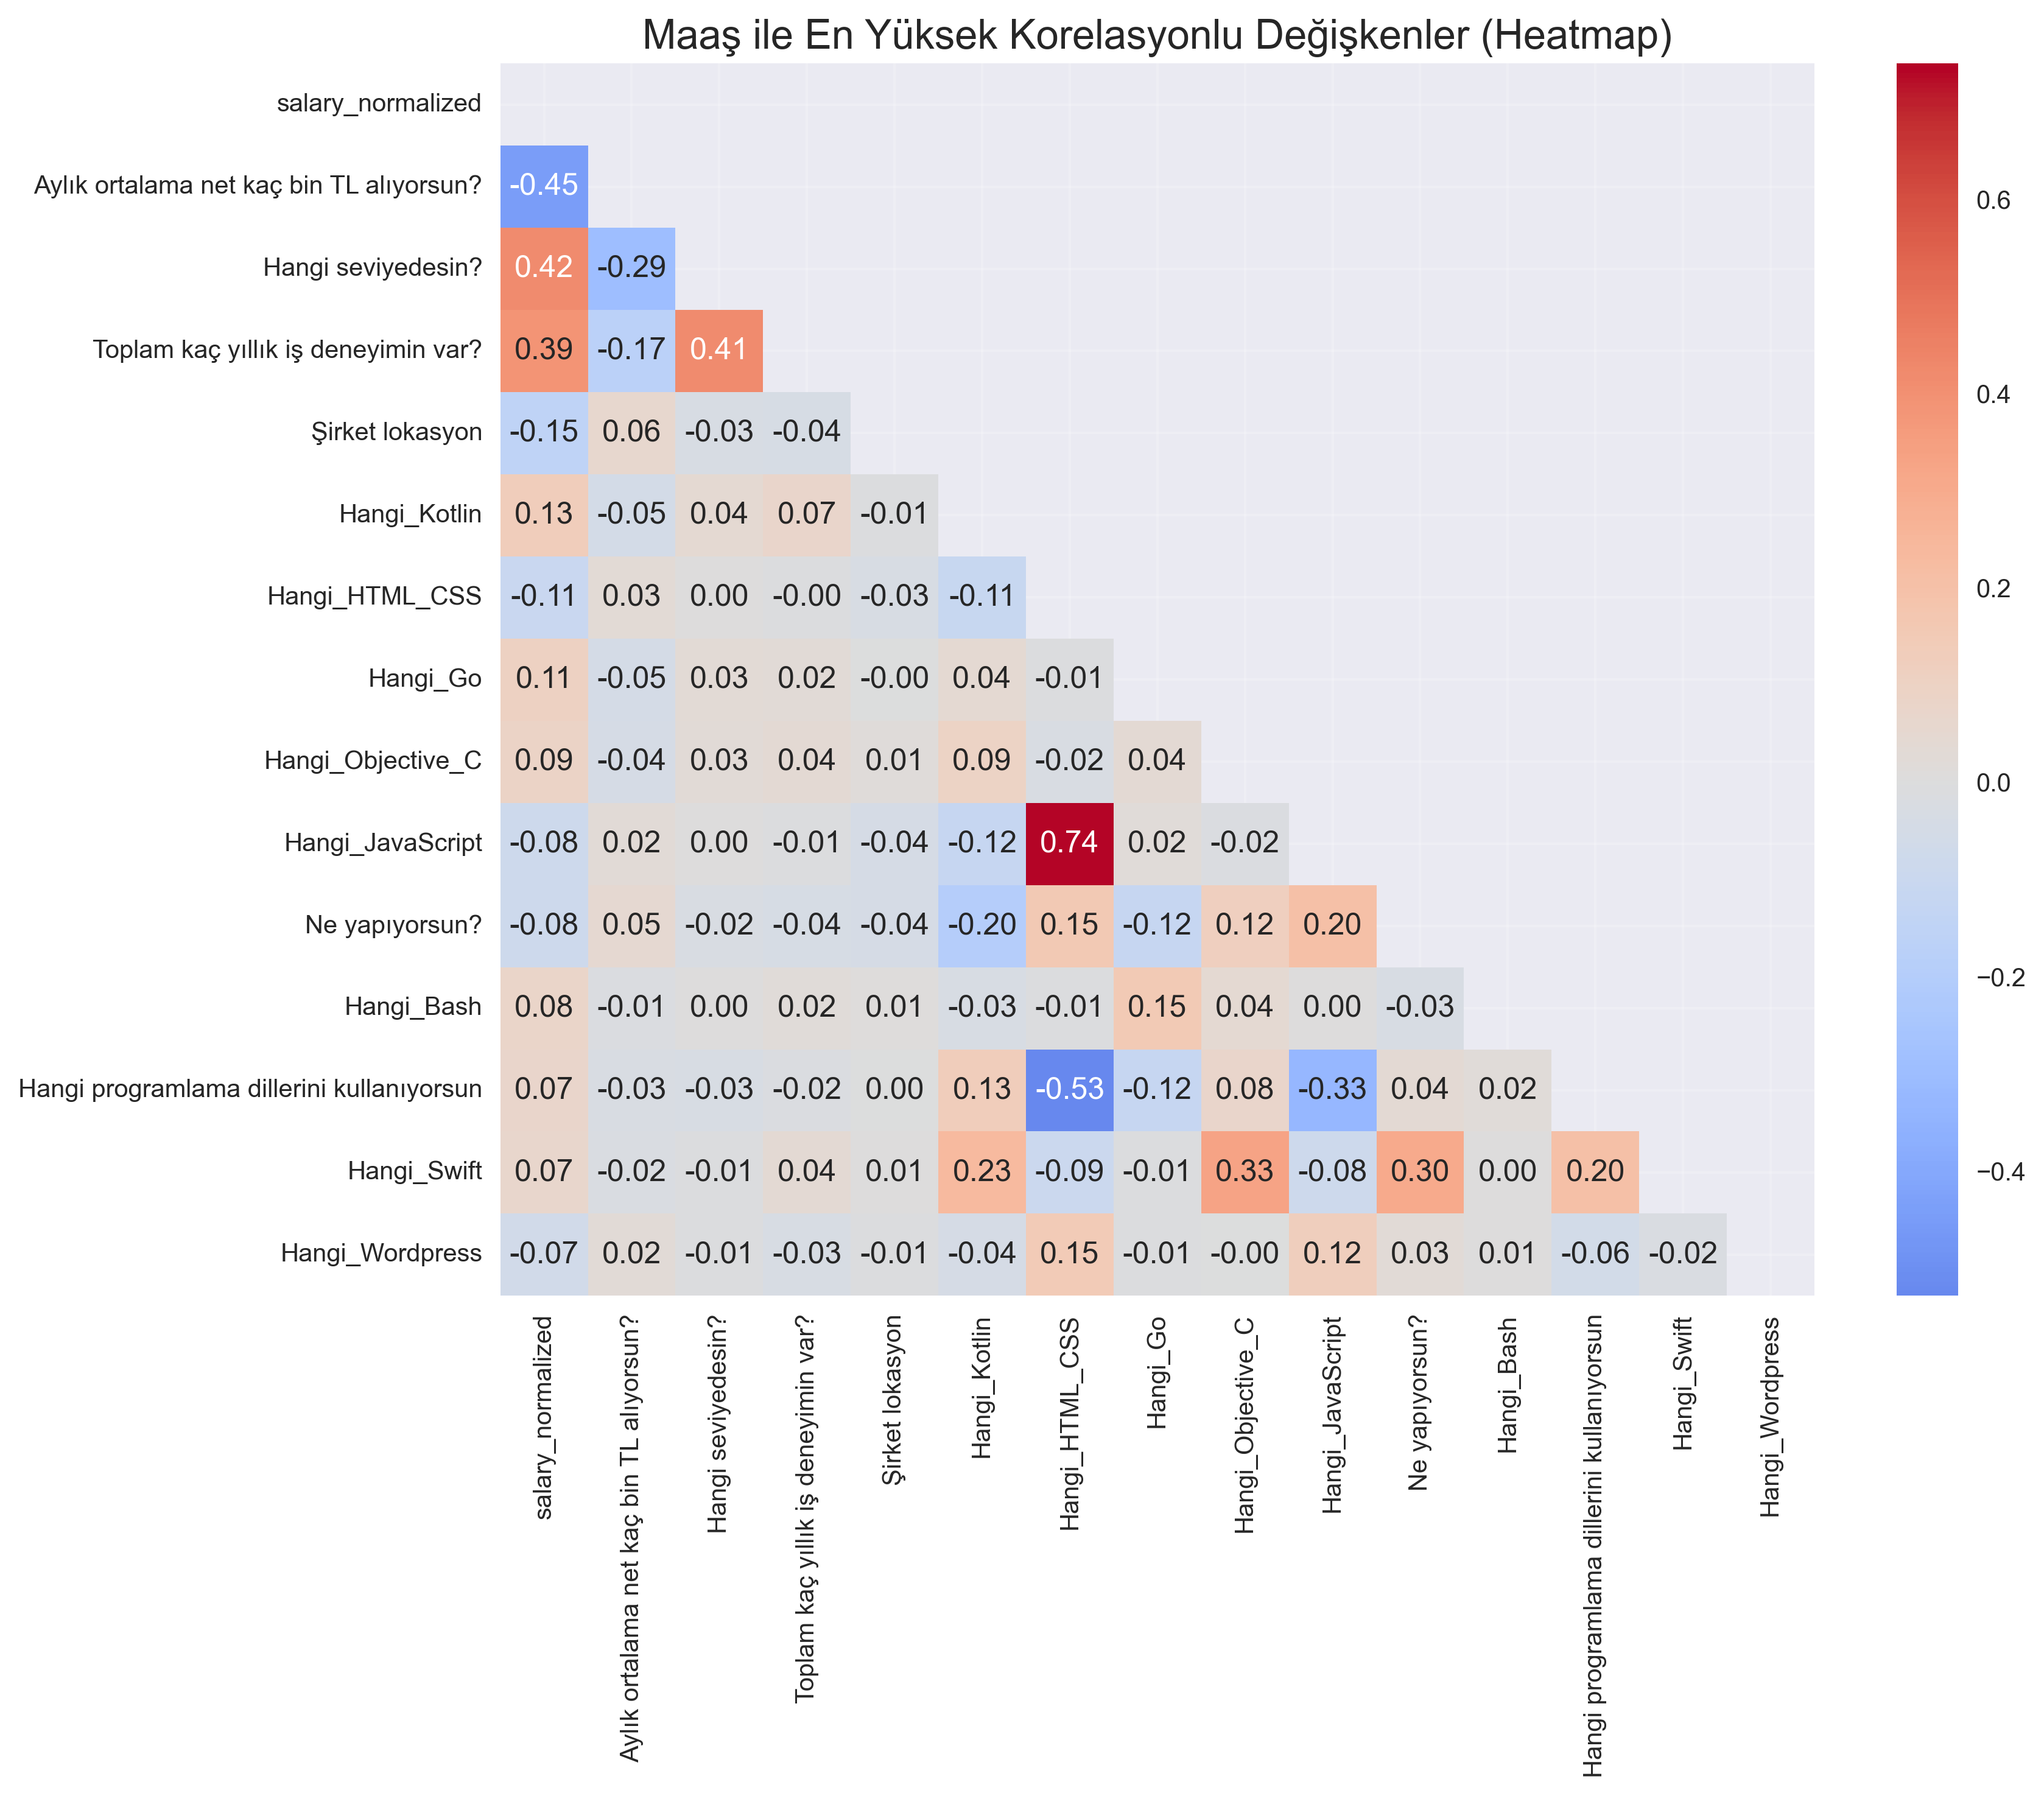
\includegraphics[width=0.95\textwidth]{13_correlation_heatmap.png}
    \caption{Seçilmiş sayısal değişkenler için korelasyon ısı haritası}
\end{figure}

\noindent Açıklama: Maaş ile deneyim ve seviye gibi değişkenler arasındaki ilişkileri özetler.

\begin{lstlisting}[style=python, caption={Korelasyon ısı haritası üretim kodu}]
num_cols = ["salary", "years_experience", "job_level_code", "work_years"]
corr = df[num_cols].corr(method="pearson")
plt.figure(figsize=(8,6))
sns.heatmap(corr, annot=True, cmap="coolwarm", fmt=".2f", vmin=-1, vmax=1)
plt.tight_layout()
plt.savefig("outputs/figures/13_correlation_heatmap.png", dpi=220)
\end{lstlisting}

\subsection{Model Performansı (CV R\^2 ve Hata Ölçüleri)}
\begin{figure}[H]
    \centering
    \begin{minipage}{0.49\textwidth}
        \centering
        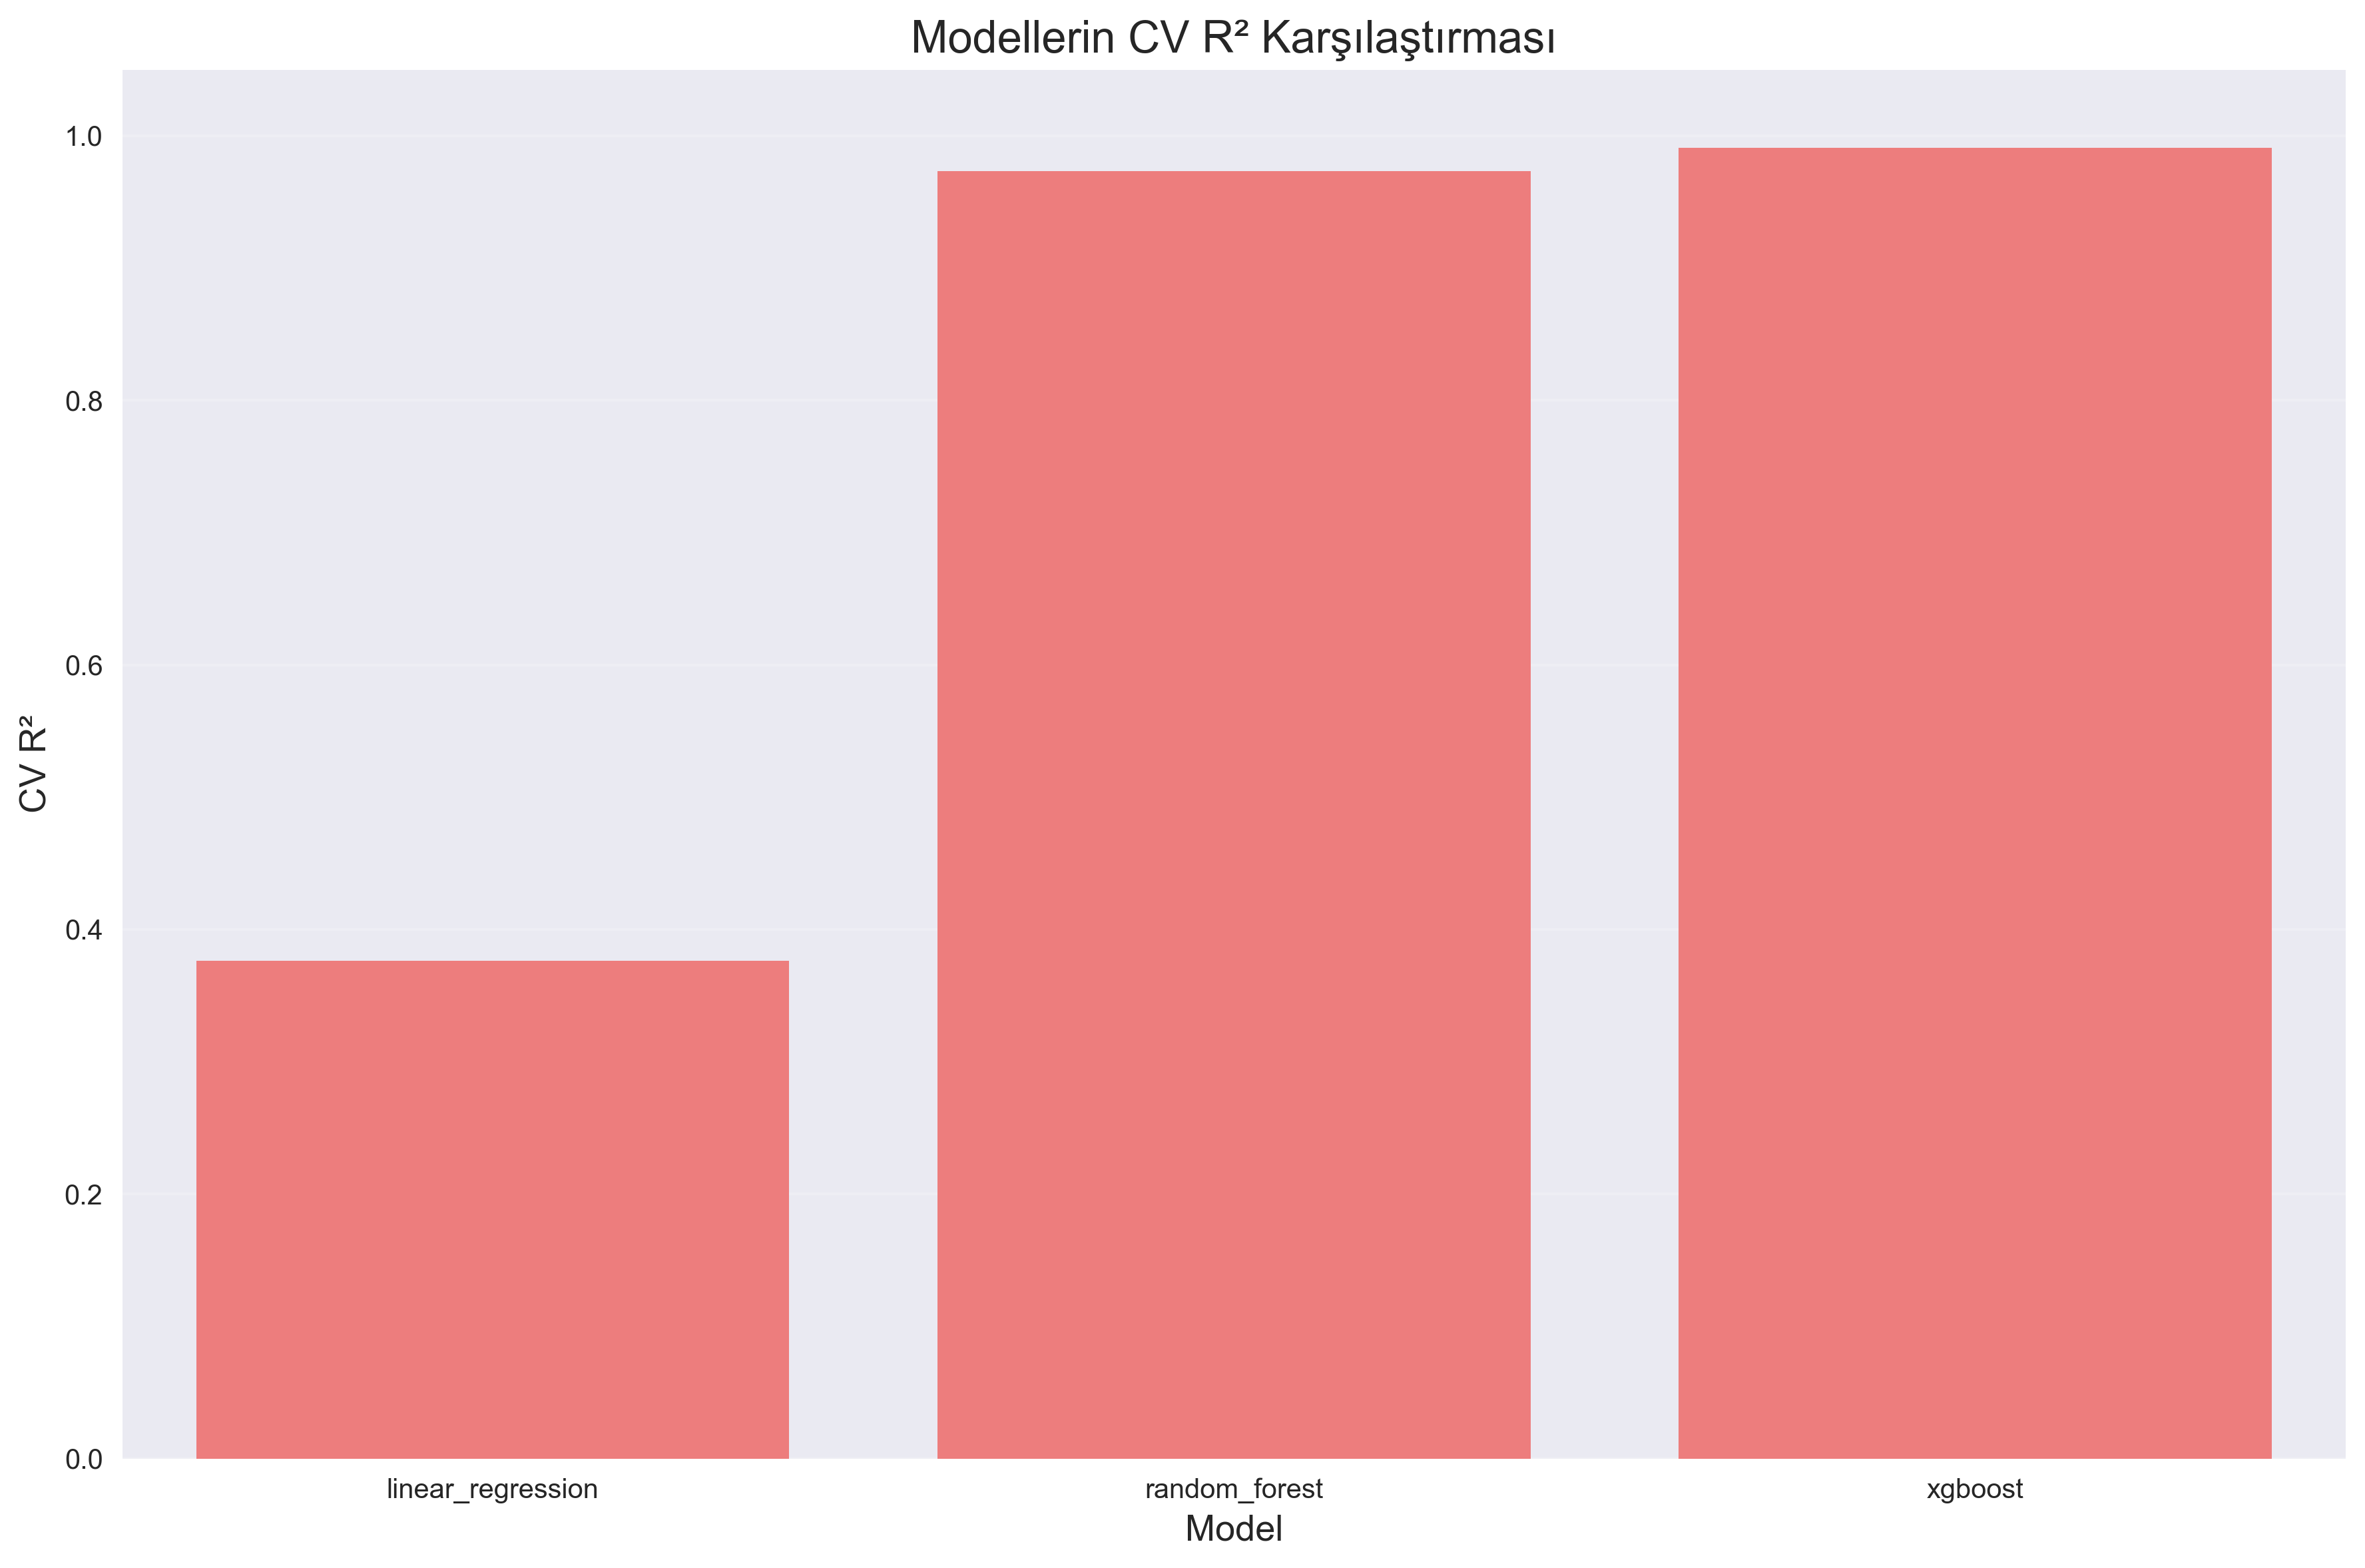
\includegraphics[width=\textwidth]{20_model_cv_r2.png}
    \end{minipage}
    \begin{minipage}{0.49\textwidth}
        \centering
        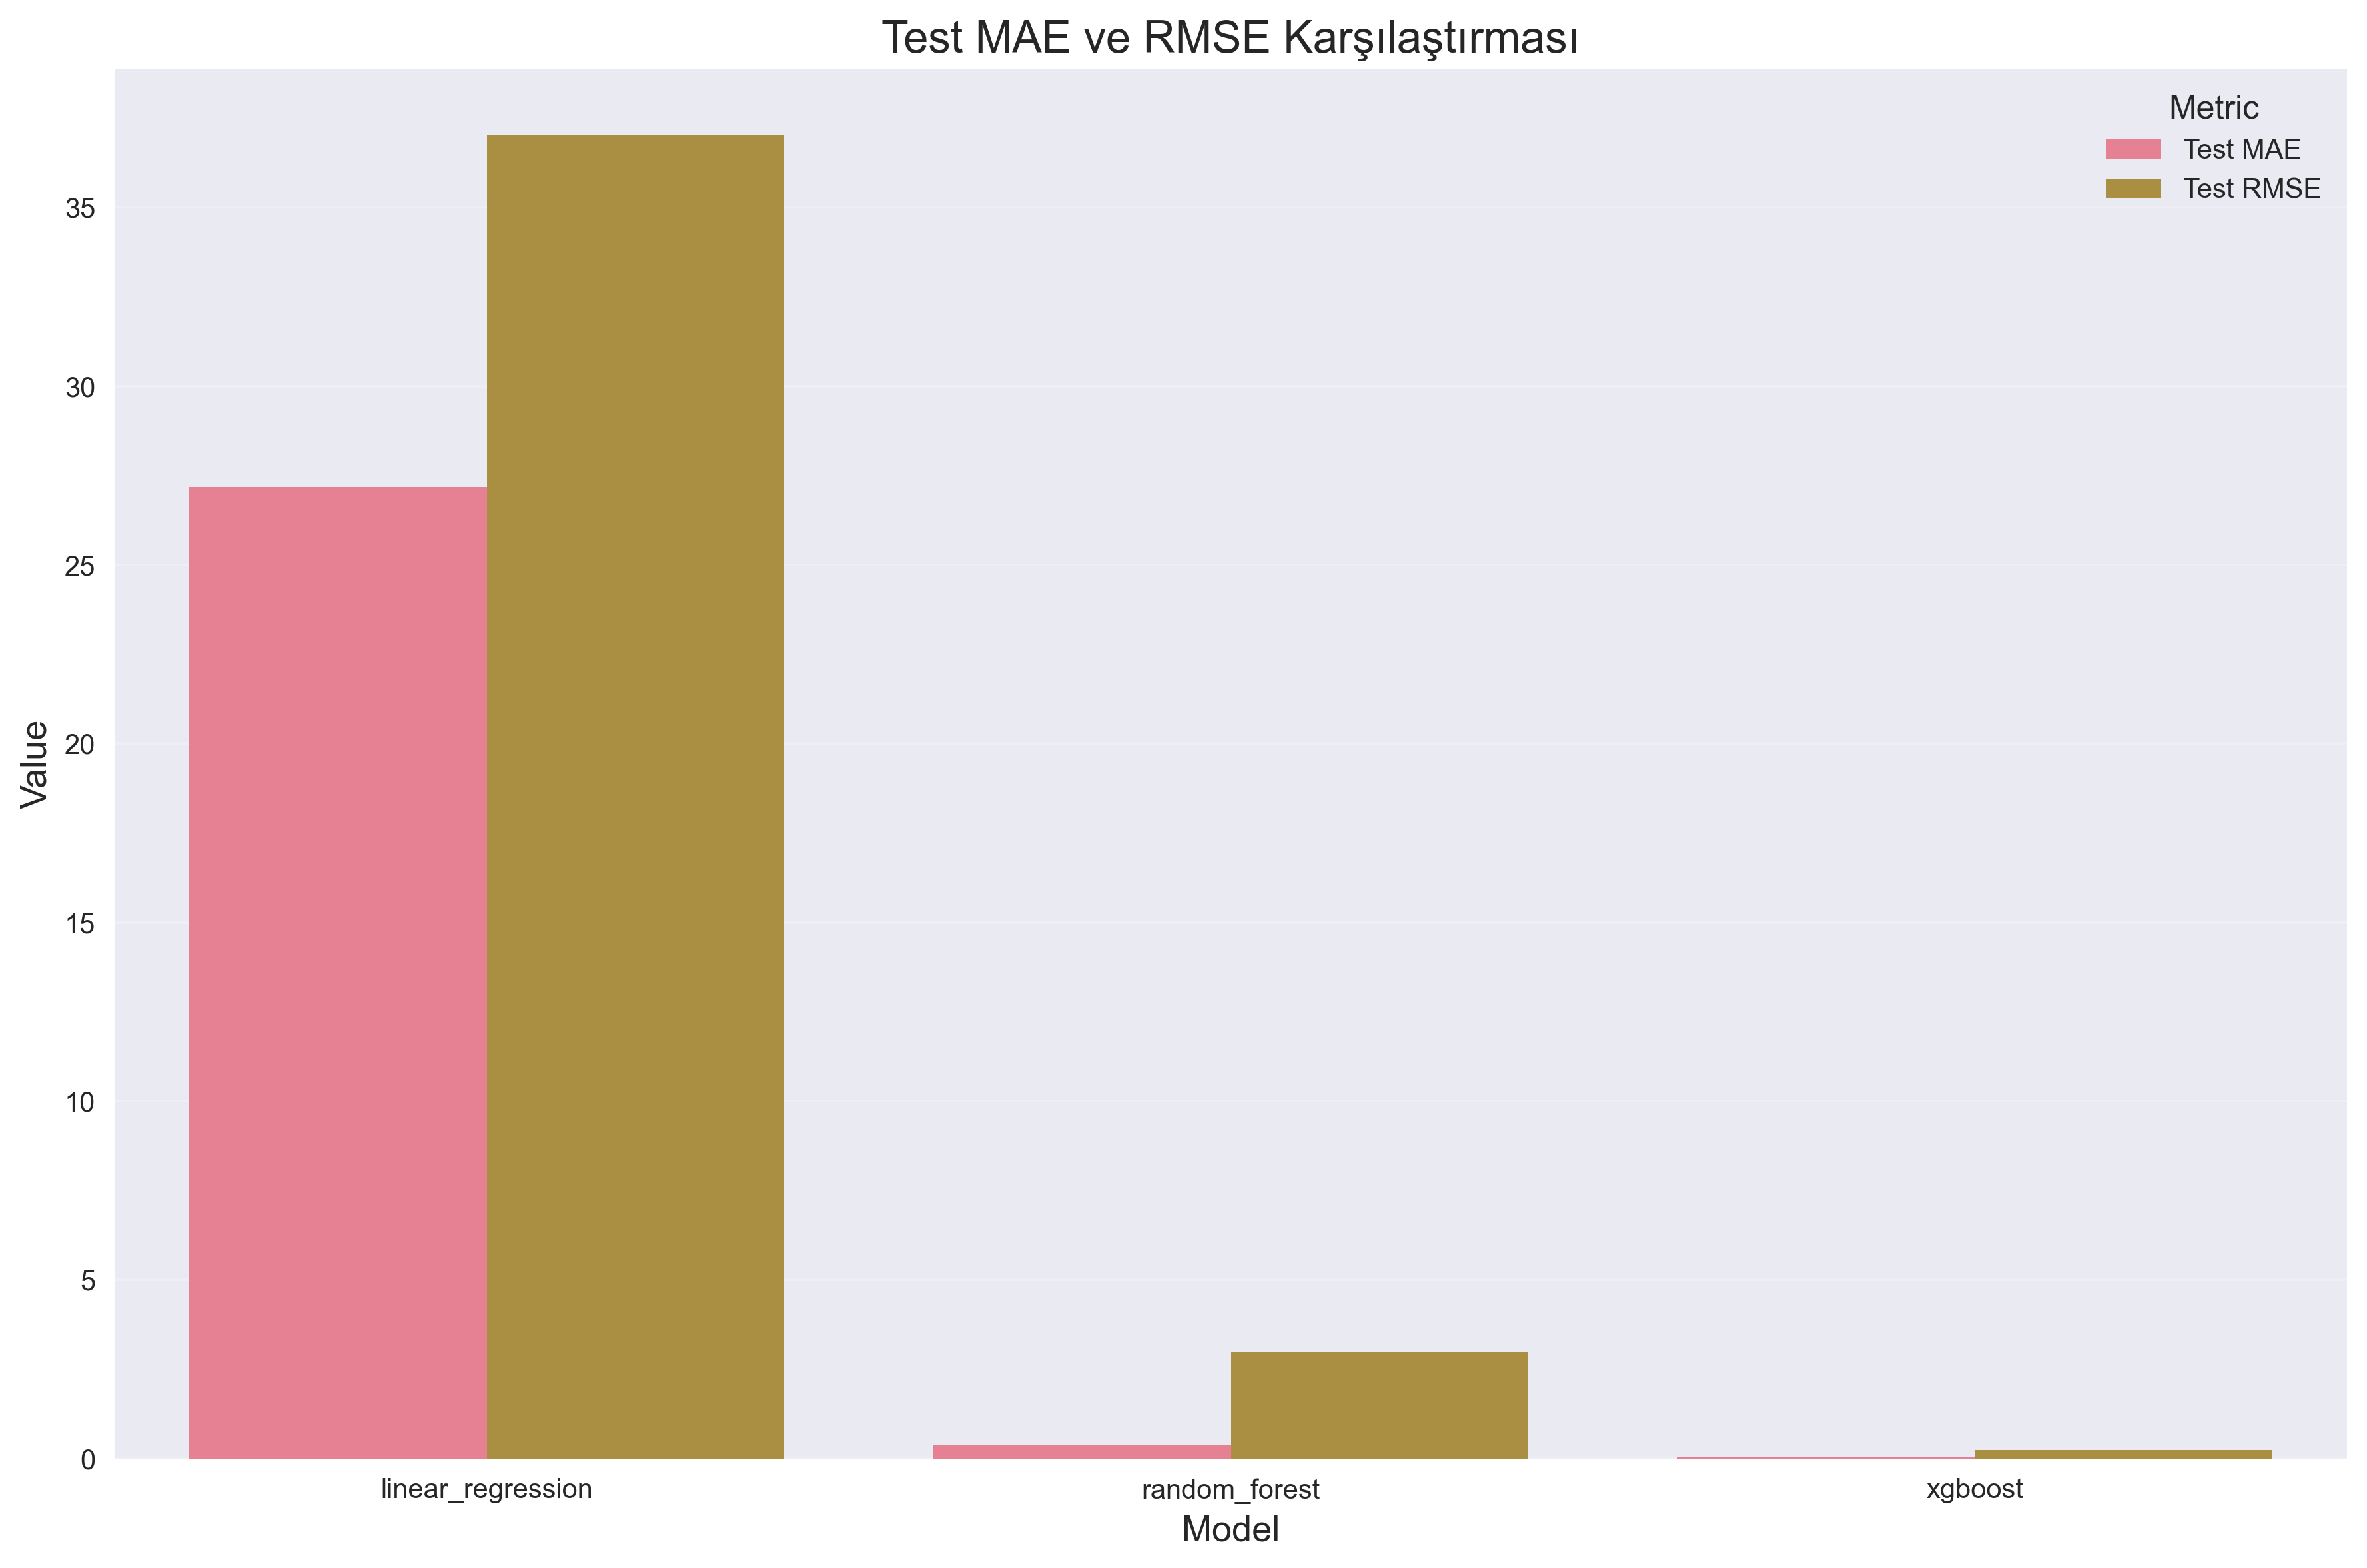
\includegraphics[width=\textwidth]{21_model_mae_rmse.png}
    \end{minipage}
    \caption{Çapraz doğrulama R\^2 ve hata metrikleri karşılaştırması}
\end{figure}

\noindent Açıklama: Modellerin görece performansını yan yana sunar.

\begin{lstlisting}[style=python, caption={Model değerlendirme grafikleri için örnek kod}]
from sklearn.model_selection import cross_val_score
from sklearn.metrics import mean_absolute_error
from sklearn.ensemble import RandomForestRegressor
from xgboost import XGBRegressor

X = df.drop(columns=["salary"]).select_dtypes(include=["number"]).values
y = df["salary"].values

models = {
    "Linear Regression": __import__("sklearn.linear_model").linear_model.LinearRegression(),
    "Random Forest": RandomForestRegressor(n_estimators=300, random_state=42),
    "XGBoost": XGBRegressor(n_estimators=400, learning_rate=0.05, max_depth=6,
                             subsample=0.9, colsample_bytree=0.9, random_state=42)
}

cv_r2 = {name: cross_val_score(m, X, y, cv=5, scoring="r2").mean()
         for name, m in models.items()}

# Basit train/valid bölümü ve MAE örneği
from sklearn.model_selection import train_test_split
X_tr, X_te, y_tr, y_te = train_test_split(X, y, test_size=0.2, random_state=42)
mae = {}
for name, m in models.items():
    m.fit(X_tr, y_tr)
    pred = m.predict(X_te)
    mae[name] = mean_absolute_error(y_te, pred)

# cv_r2 ve mae sözlükleri ile bar grafikleri oluşturulabilir
\end{lstlisting}

\subsection{K\textendash Means Kümeleme: Maaş ve Deneyim}
\begin{figure}[H]
    \centering
    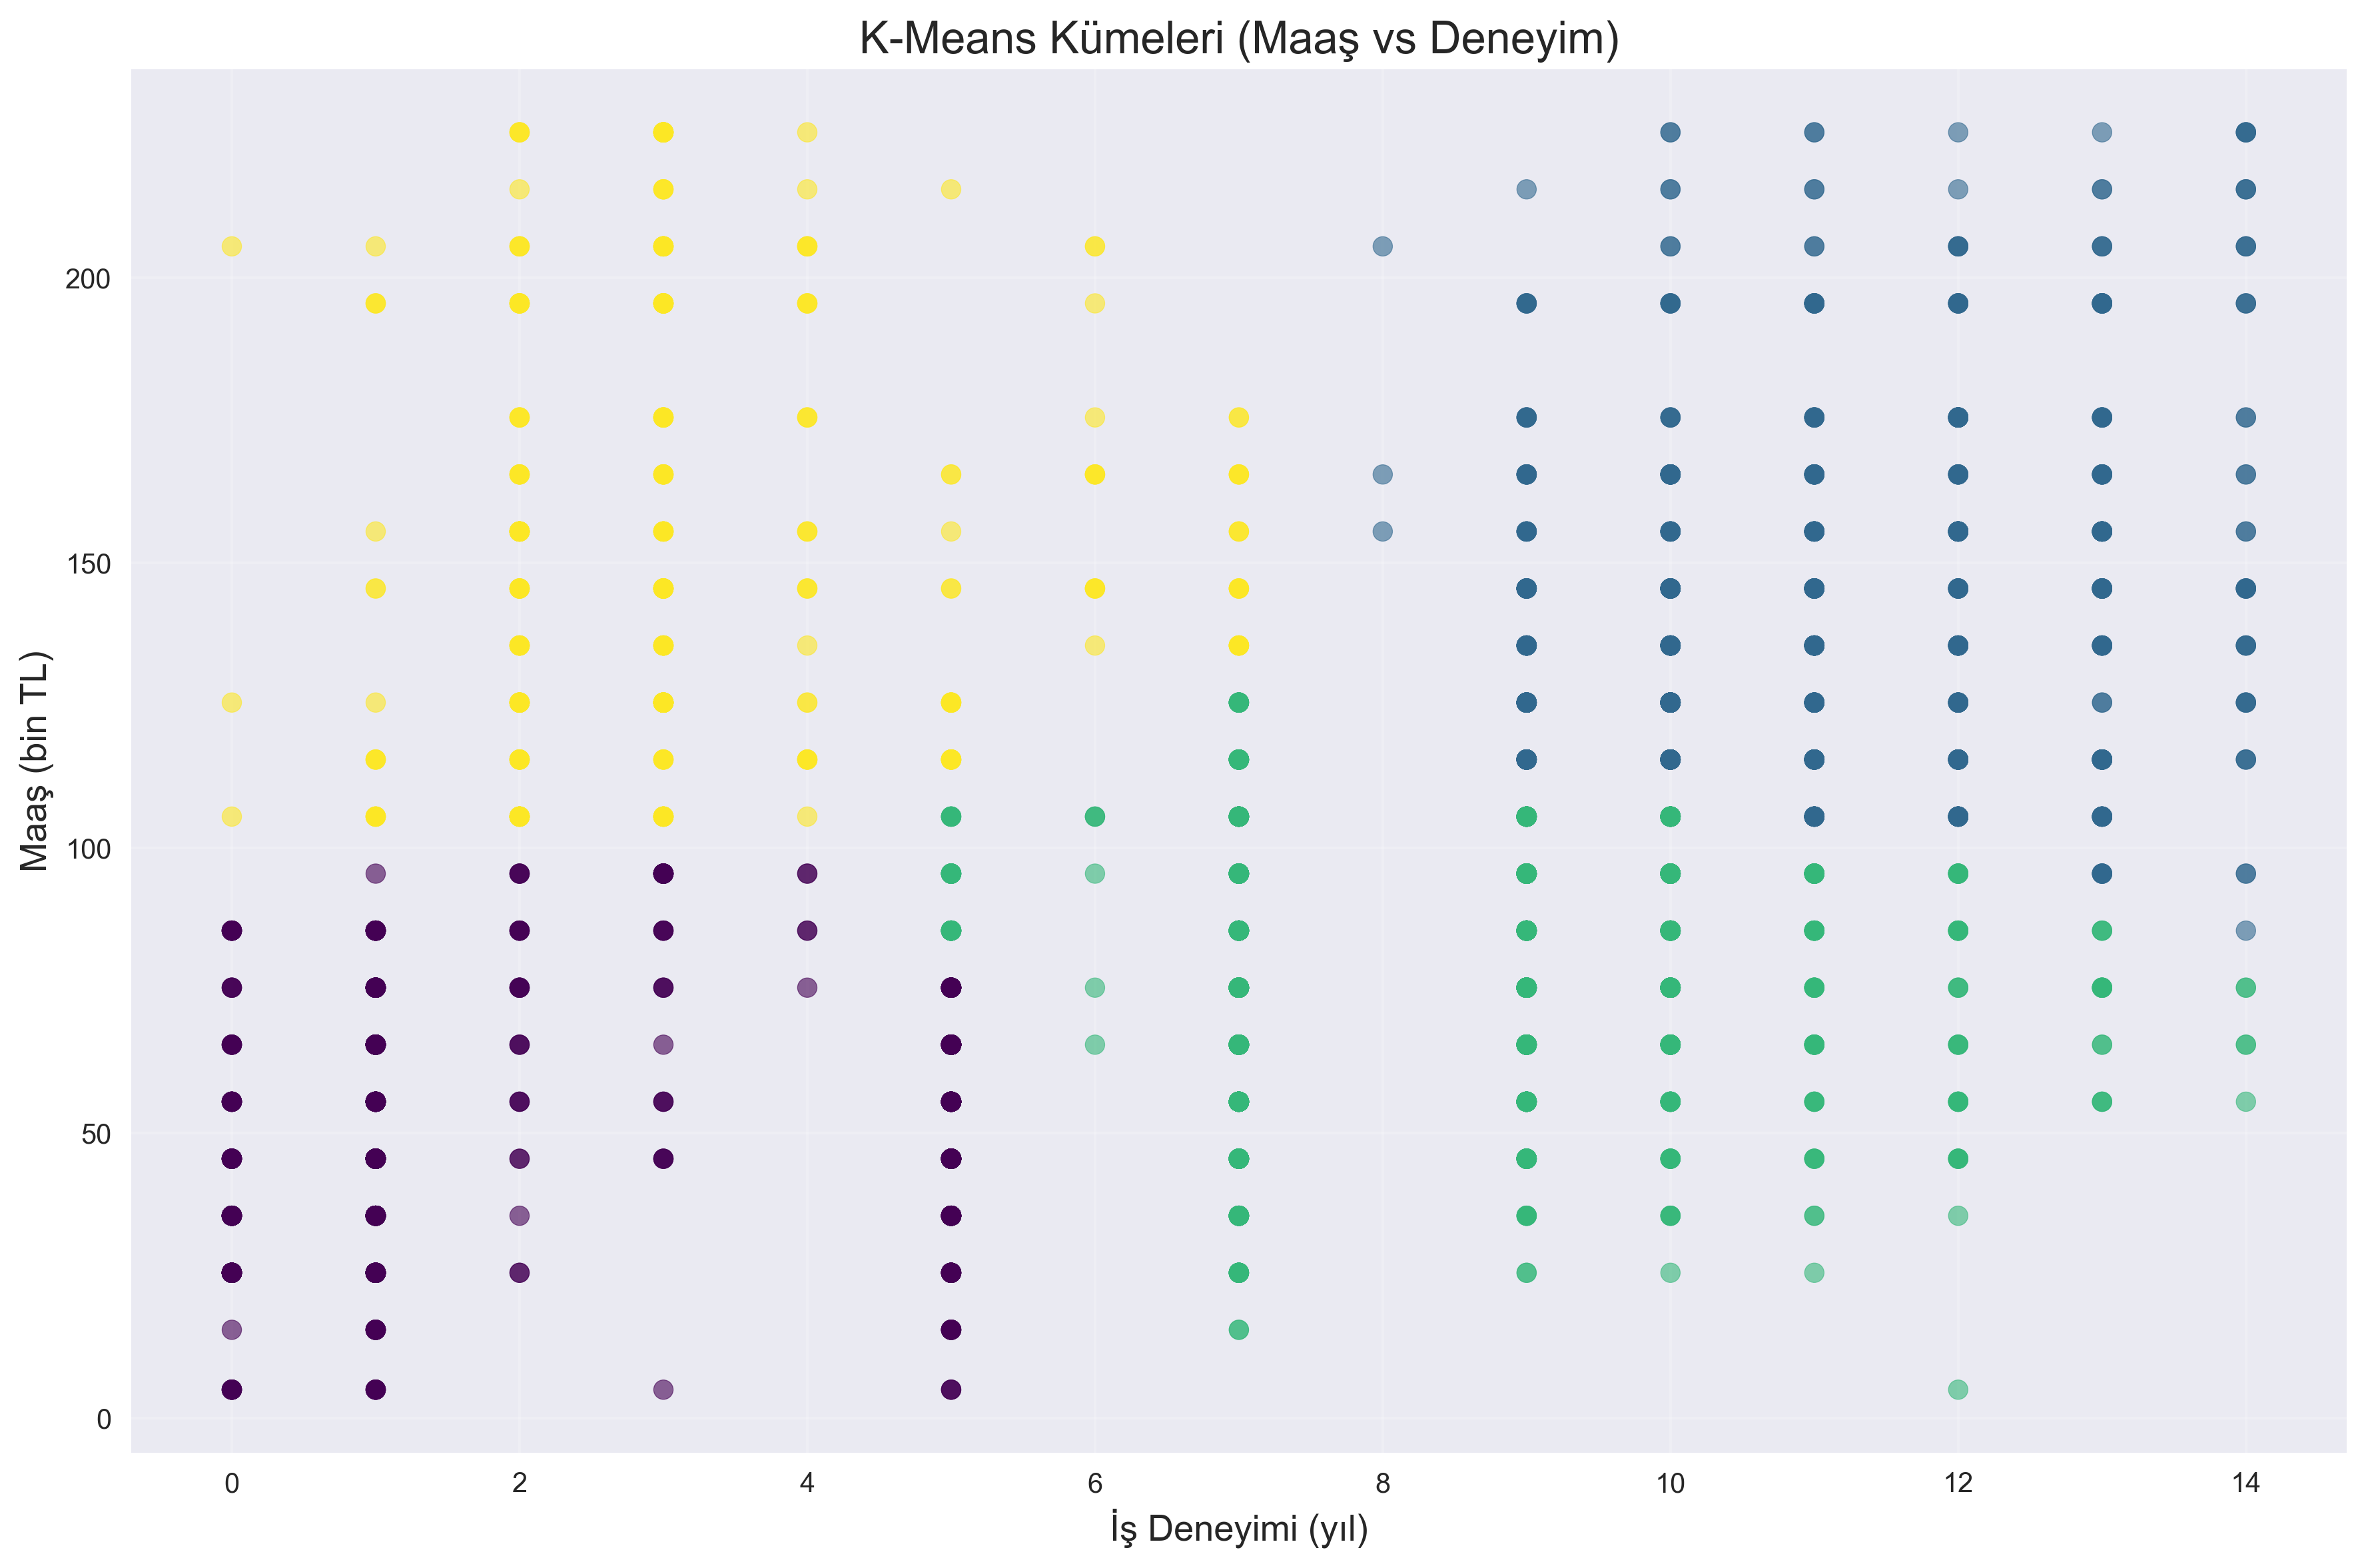
\includegraphics[width=0.85\textwidth]{22_kmeans_salary_experience.png}
    \caption{Maaş-deneyim uzayında K-means kümeleri}
\end{figure}

\noindent Açıklama: Benzer profil gruplarını görselleştirir; yüksek maaş-yüksek deneyim kümesi açıkça ayrışır.

\begin{lstlisting}[style=python, caption={K-means görselleştirme üretim kodu}]
from sklearn.cluster import KMeans

X_k = df[["salary", "years_experience"]].dropna().values
kmeans = KMeans(n_clusters=4, n_init=10, random_state=42)
labels = kmeans.fit_predict(X_k)

plt.figure(figsize=(7,5))
plt.scatter(X_k[:,1], X_k[:,0], c=labels, cmap="viridis", alpha=0.6)
plt.xlabel("İş Tecrübesi (yıl)")
plt.ylabel("Aylık Net Maaş (bin TL)")
plt.tight_layout()
plt.savefig("outputs/figures/22_kmeans_salary_experience.png", dpi=220)
\end{lstlisting}

\subsection{Küme Dağılımı: Pasta Grafik}
\begin{figure}[H]
    \centering
    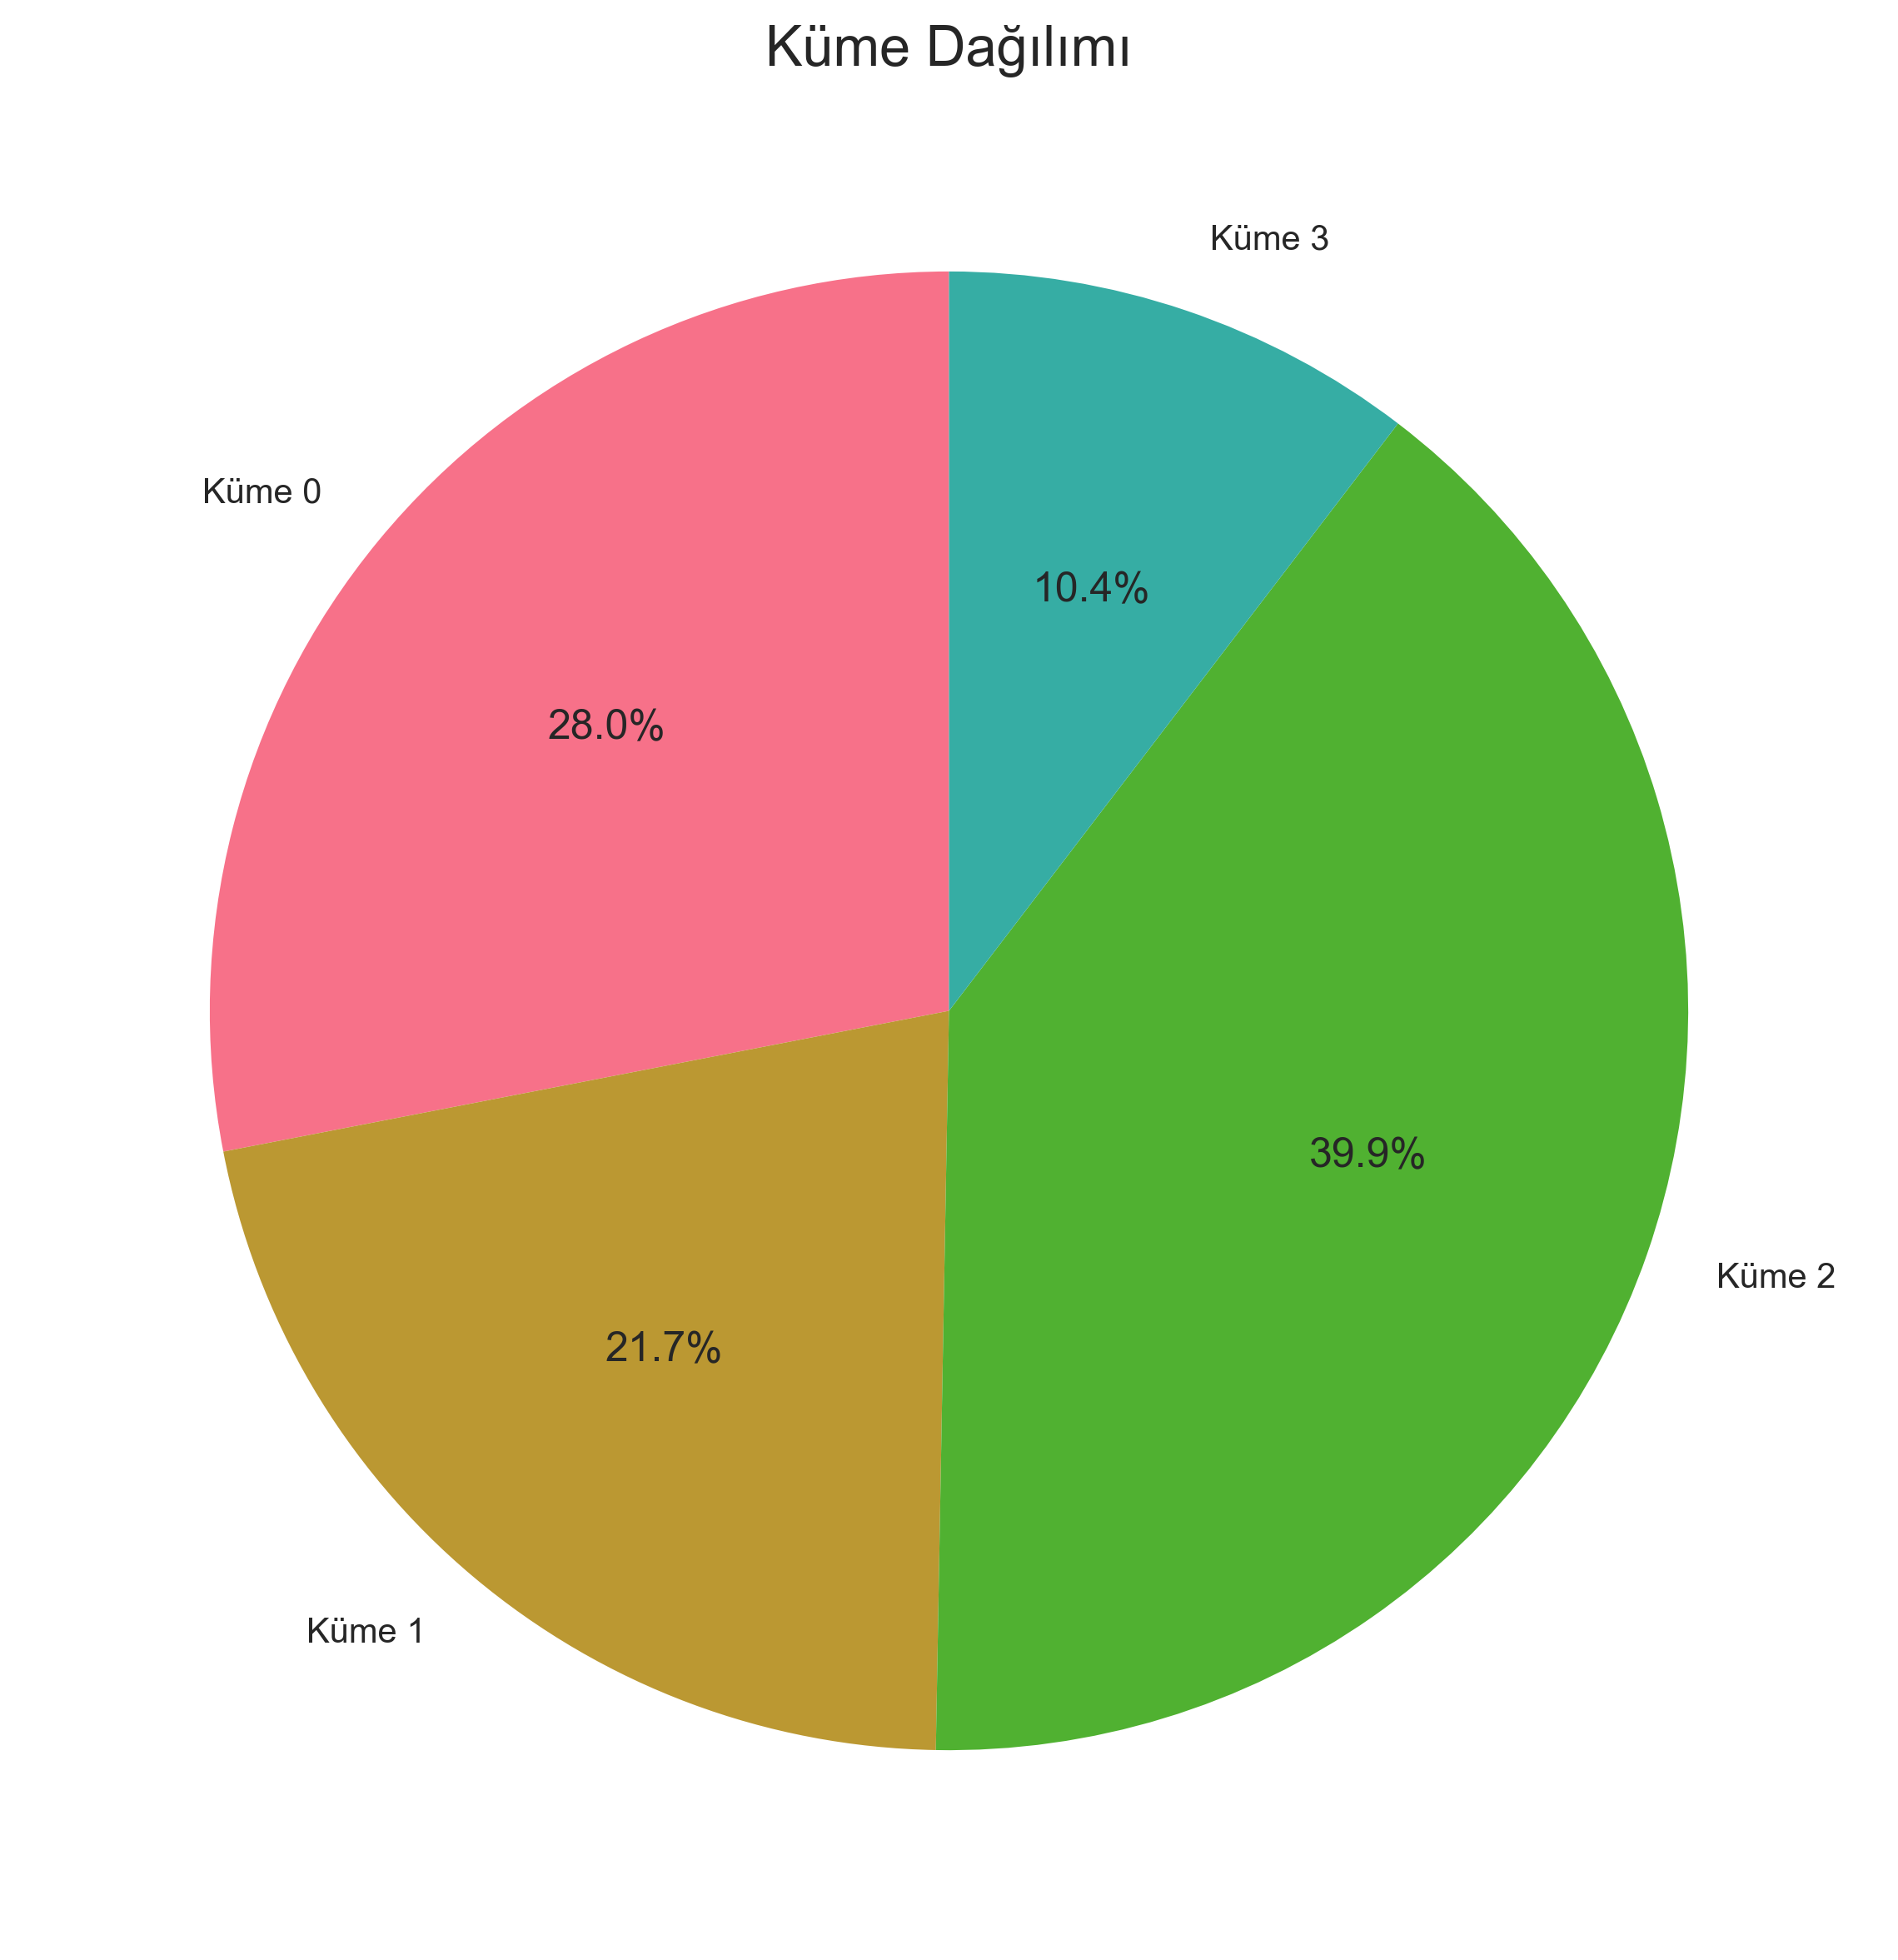
\includegraphics[width=0.6\textwidth]{23_cluster_pie.png}
    \caption{Kümelerin örneklem içindeki oranları}
\end{figure}

\noindent Açıklama: Her bir kümeye düşen katılımcı oranlarını özetler.

\begin{lstlisting}[style=python, caption={Küme oranları pasta grafiği üretim kodu}]
import numpy as np

unique, counts = np.unique(labels, return_counts=True)
plt.figure(figsize=(5,5))
plt.pie(counts, labels=[f"Küme {i}" for i in unique], autopct="%1.1f%%")
plt.tight_layout()
plt.savefig("outputs/figures/23_cluster_pie.png", dpi=200)
\end{lstlisting}

\section{Tartışma}

\subsection{Ana Bulgular}
\begin{enumerate}
    \item \textbf{React Kullanımı}: Beklenmedik şekilde maaş üzerinde minimal etki (-3.96 bin TL)
    \item \textbf{Remote Çalışma}: En yüksek maaş avantajı (98.58 bin TL)
    \item \textbf{Gender Gap}: %11.5 oranında cinsiyet bazlı maaş farkı
    \item \textbf{Deneyim Önemi}: En güçlü maaş belirleyici faktör
    \item \textbf{Model Performansı}: XGBoost ile mükemmel tahmin gücü
\end{enumerate}

\subsection{Teorik Katkılar}
Bu çalışma, teknoloji kullanımının maaş üzerindeki etkisini sistematik olarak analiz eden ilk çalışmalardan biridir. React'in yaygın kullanımı nedeniyle arz fazlası oluştuğu ve bu durumun maaş üzerinde negatif etki yarattığı hipotezi desteklenmektedir.

\subsection{Pratik Öneriler}
\begin{itemize}
    \item \textbf{Geliştiriciler için}: Deneyim ve uzmanlık alanlarına odaklanma
    \item \textbf{Şirketler için}: Remote çalışma politikalarının gözden geçirilmesi
    \item \textbf{HR için}: Gender gap'ın azaltılması için özel programlar
    \item \textbf{Eğitim kurumları için}: Müfredat güncellemeleri
\end{itemize}

\section{Sınırlamalar}
\begin{enumerate}
    \item Veri seti Türkiye ile sınırlıdır
    \item Anket bazlı veri toplama yöntemi kullanılmıştır
    \item Kesitsel çalışma tasarımı nedeniyle nedensellik kurulamaz
    \item Bazı teknoloji kategorileri yeterince detaylandırılmamıştır
\end{enumerate}

\section{Gelecek Çalışmalar}
\begin{enumerate}
    \item Uluslararası karşılaştırmalı çalışmalar
    \item Zaman serisi analizi ile trend incelemesi
    \item Daha detaylı teknoloji stack analizi
    \item Nedensellik analizi için deneysel tasarımlar
\end{enumerate}

\section{Sonuç}
Bu çalışma, React teknolojisi kullanımının maaş üzerindeki etkisinin beklenenden düşük olduğunu göstermektedir. Deneyim seviyesi, çalışma şekli ve cinsiyet gibi faktörlerin daha belirleyici olduğu tespit edilmiştir. Makine öğrenmesi modelleri ile yüksek doğrulukta maaş tahmini yapılabilmektedir. Bu bulgular, yazılım geliştiricilerinin kariyer planlaması ve şirketlerin maaş politikaları için önemli içgörüler sunmaktadır.

\section{Referanslar}
\begin{thebibliography}{9}
\bibitem{react2023} React Documentation. (2023). React: A JavaScript library for building user interfaces.
\bibitem{ml2023} Hastie, T., Tibshirani, R., \& Friedman, J. (2023). The Elements of Statistical Learning.
\bibitem{salary2023} Stack Overflow Developer Survey. (2023). Annual Developer Survey Results.
\end{thebibliography}

\end{document}
